\subsection{A fresh look}
Plots of observed and fitted values can tell part of the story,
but it is the \emph{comparison} of the two, in relation to the structure of
the data, which is most effective in suggesting ways to modify a
given model.  Probability plots or index plots of residuals can be useful,
but these do not relate to the structure of the contingency table
or to the pattern of association.
Mosaic displays and \CA\ are more useful for understanding the nature of associations,
which they reveal in different ways.

\begin{Example}[vietnam2]{Student opinion about the Vietnam war}
Because we have seen that the associations of response with year
differ for men and women, it is natural to examine partial mosaic
plots for the two sexes.
This is easily done with the \macro{MOSAIC}, using \pname{by=sex}.
First, a \Dstp\ is used to create more meaningful labels for
\pname{response} and \pname{year}. These statements create the two
graphs shown in \figref{fig:mosviet}.
\subsection{A fresh look}
Plots of observed and fitted values can tell part of the story,
but it is the \emph{comparison} of the two, in relation to the structure of
the data, which is most effective in suggesting ways to modify a
given model.  Probability plots or index plots of residuals can be useful,
but these do not relate to the structure of the contingency table
or to the pattern of association.
Mosaic displays and \CA\ are more useful for understanding the nature of associations,
which they reveal in different ways.

\begin{Example}[vietnam2]{Student opinion about the Vietnam war}
Because we have seen that the associations of response with year
differ for men and women, it is natural to examine partial mosaic
plots for the two sexes.
This is easily done with the \macro{MOSAIC}, using \pname{by=sex}.
First, a \Dstp\ is used to create more meaningful labels for
\pname{response} and \pname{year}. These statements create the two
graphs shown in \figref{fig:mosviet}.
\subsection{A fresh look}
Plots of observed and fitted values can tell part of the story,
but it is the \emph{comparison} of the two, in relation to the structure of
the data, which is most effective in suggesting ways to modify a
given model.  Probability plots or index plots of residuals can be useful,
but these do not relate to the structure of the contingency table
or to the pattern of association.
Mosaic displays and \CA\ are more useful for understanding the nature of associations,
which they reveal in different ways.

\begin{Example}[vietnam2]{Student opinion about the Vietnam war}
Because we have seen that the associations of response with year
differ for men and women, it is natural to examine partial mosaic
plots for the two sexes.
This is easily done with the \macro{MOSAIC}, using \pname{by=sex}.
First, a \Dstp\ is used to create more meaningful labels for
\pname{response} and \pname{year}. These statements create the two
graphs shown in \figref{fig:mosviet}.
\subsection{A fresh look}
Plots of observed and fitted values can tell part of the story,
but it is the \emph{comparison} of the two, in relation to the structure of
the data, which is most effective in suggesting ways to modify a
given model.  Probability plots or index plots of residuals can be useful,
but these do not relate to the structure of the contingency table
or to the pattern of association.
Mosaic displays and \CA\ are more useful for understanding the nature of associations,
which they reveal in different ways.

\begin{Example}[vietnam2]{Student opinion about the Vietnam war}
Because we have seen that the associations of response with year
differ for men and women, it is natural to examine partial mosaic
plots for the two sexes.
This is easily done with the \macro{MOSAIC}, using \pname{by=sex}.
First, a \Dstp\ is used to create more meaningful labels for
\pname{response} and \pname{year}. These statements create the two
graphs shown in \figref{fig:mosviet}.
\input{ch7/sas/mosviet}

%% two subfig side-by-side
\begin{figure}[htb]
 \begin{minipage}[t]{.49\linewidth}
  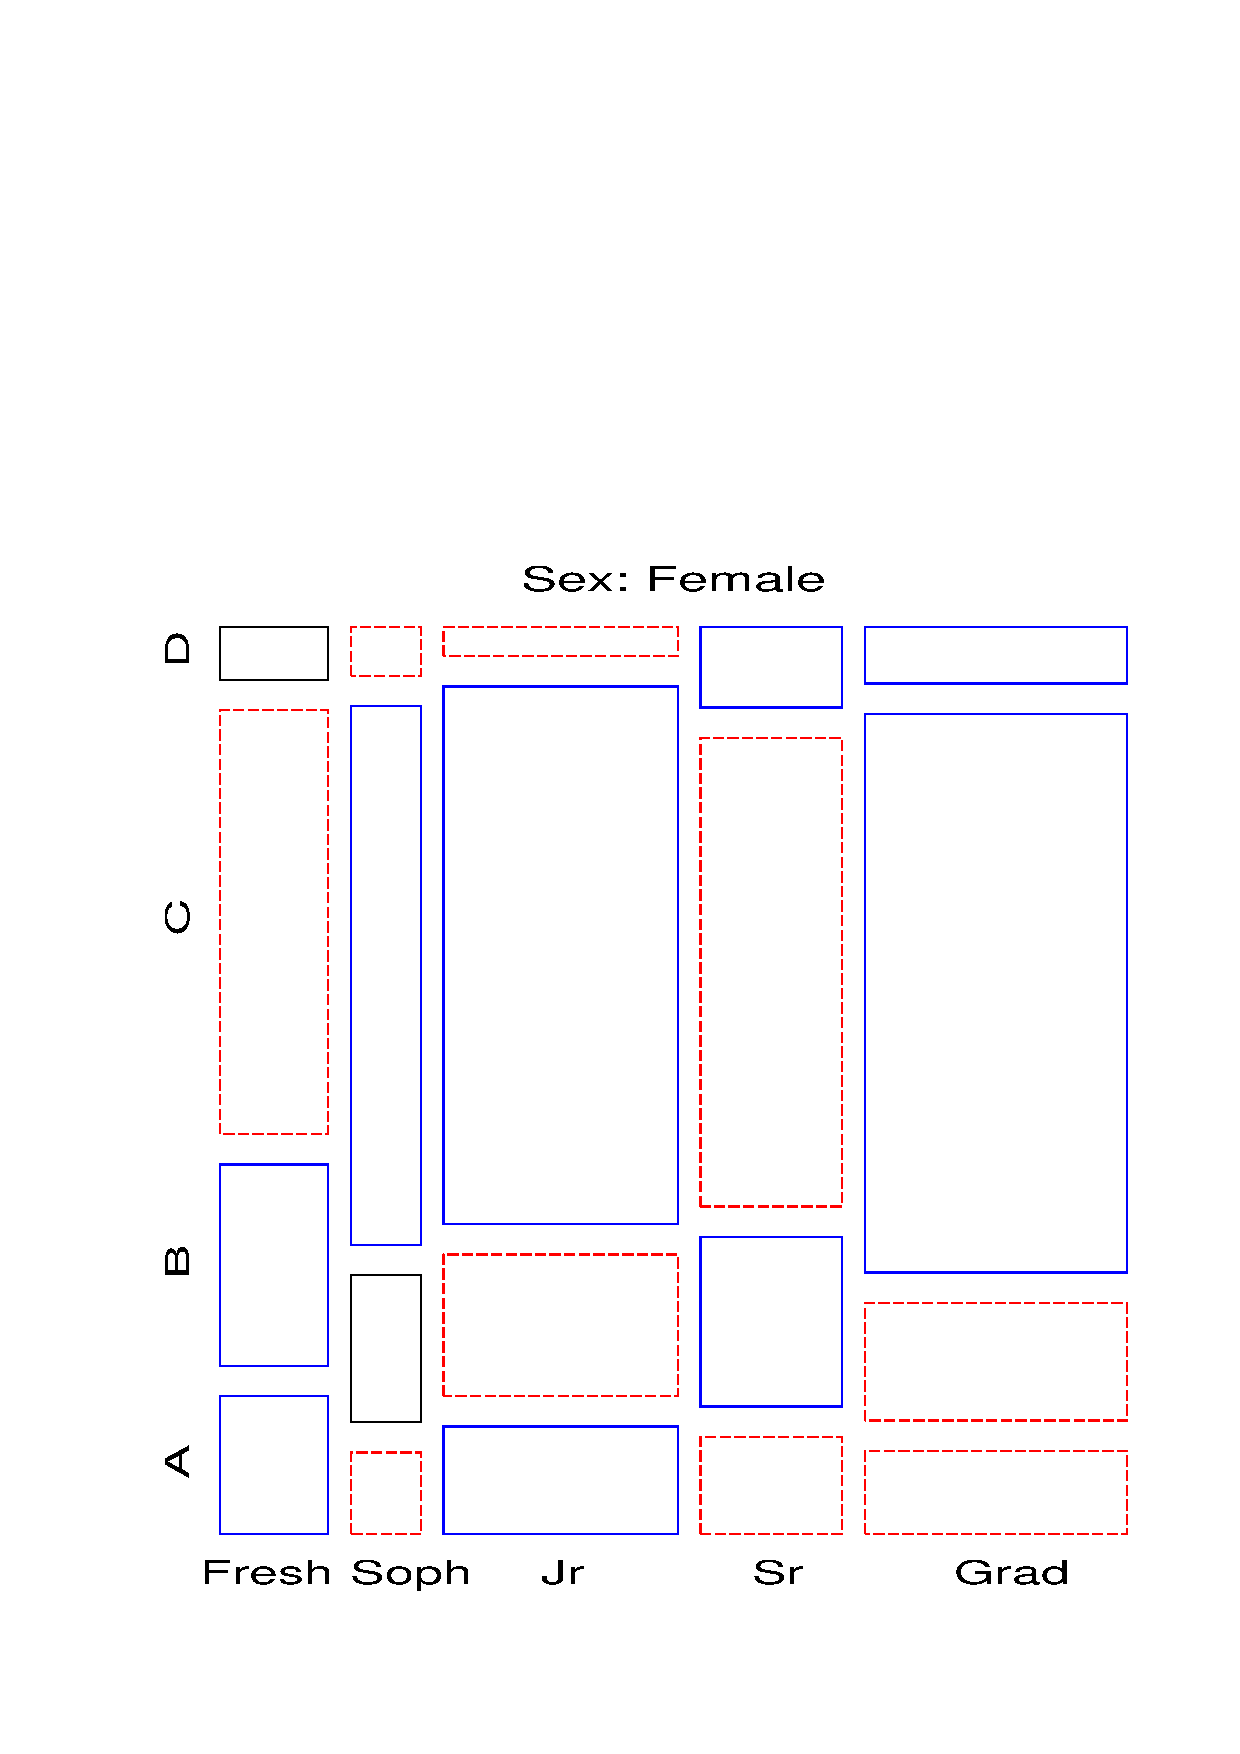
\includegraphics[width=1\linewidth,clip]{mosviet1}
 \end{minipage}%
 \hfill
 \begin{minipage}[t]{.49\linewidth}
  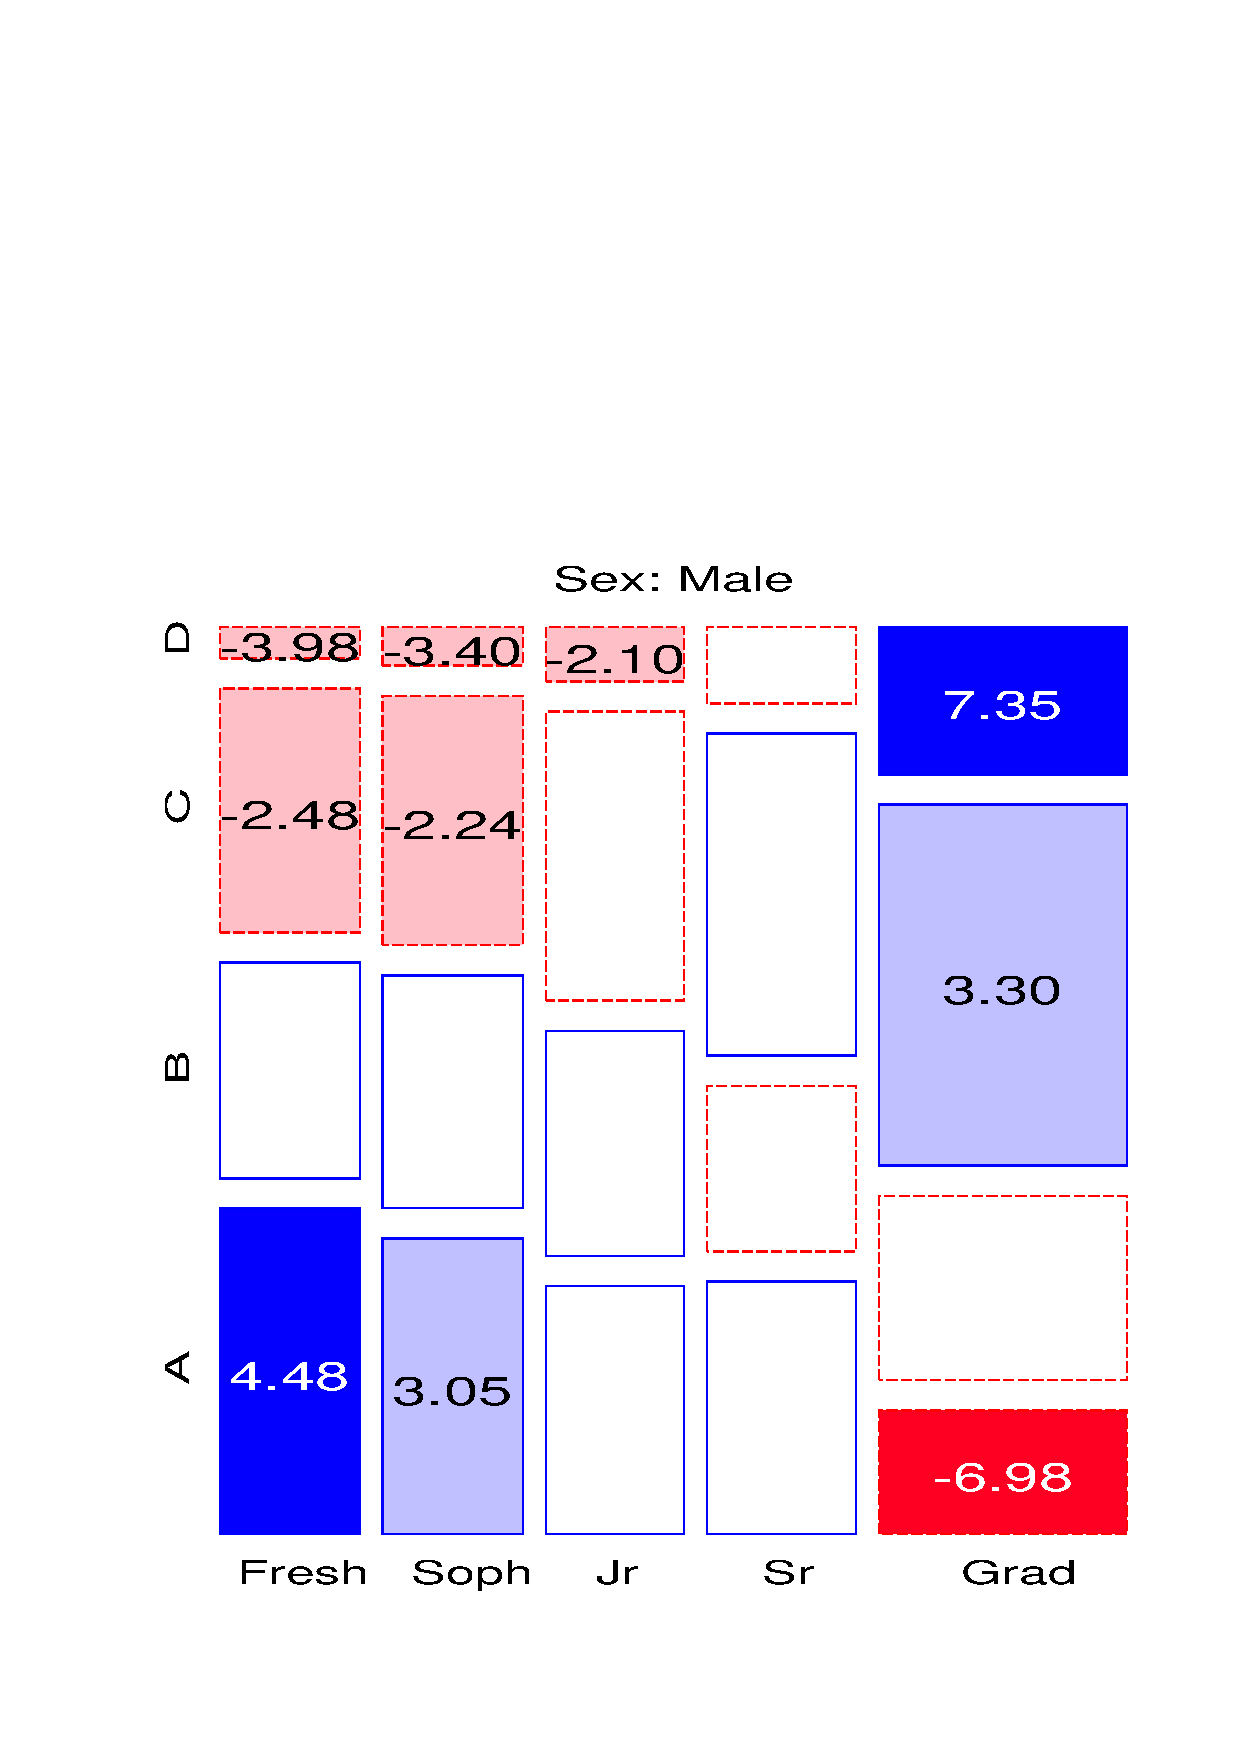
\includegraphics[width=1\linewidth,clip]{mosviet2}
 \end{minipage}
 \caption{Partial mosaic plots, by sex, for Vietnam war data}\label{fig:mosviet}
\end{figure}
With the variables in each mosaic ordered Year, Response,
recall that the height of each bar shows the (conditional) proportion
of students in each year who chose each response. There is no systematic
pattern for women, but the pattern of heights of the boxes, and of the
residuals from independence for men is very systematic.
The trend over years is easiest to see for responses A and D;
note that there is a large jump in proportion choosing these responses
between 4th year students and graduate students.
Perhaps our assumption of a linear trend with year for males needs
adjustment.

A \CA\ plot also displays residuals from a background model.  Here
we choose the null-response model of joint independence, $[SY] [R]$, so that all associations
between the response and the sex-year combinations will be shown.
To do this, we first transpose the data so that the responses
are columns and the sex-year populations are rows.
\begin{listing}
%include catdata(vietnam);

*-- Reshape to two-way table, SexYr x Response;
proc transpose data=vietnam prefix=R out=viet2way;
   var count;
   by sex year;

data viet2way;
   set viet2way;
   rename r1=A r2=B r3=C r4=D;
   sexyr = sex || put(year,1.);
   drop _name_;
proc print;

%corresp(data=viet2way, var=A--D, id=sexyr, interp=none join);
\end{listing}

The plot, shown in \figref{fig:vietcores} is quite revealing.
The response points, A--D
largely define the first dimension,
which accounts for 73.6\% of the association from the null-response model.
The year points for men, M1--M5,
are also ordered along this dimension, but male graduate students are far
from the male undergraduates.
The year points for women are tightly clustered, and aligned closest to
response C, their most preferred alternative.
The second dimension seems largely to do with the contrast between the relatively high choice for response D (``immediate withdrawal'')
among male graduate students and general preference for response C
(``de-escalate'') among most women.

%% one figure
\begin{figure}[htb]
  \centering
  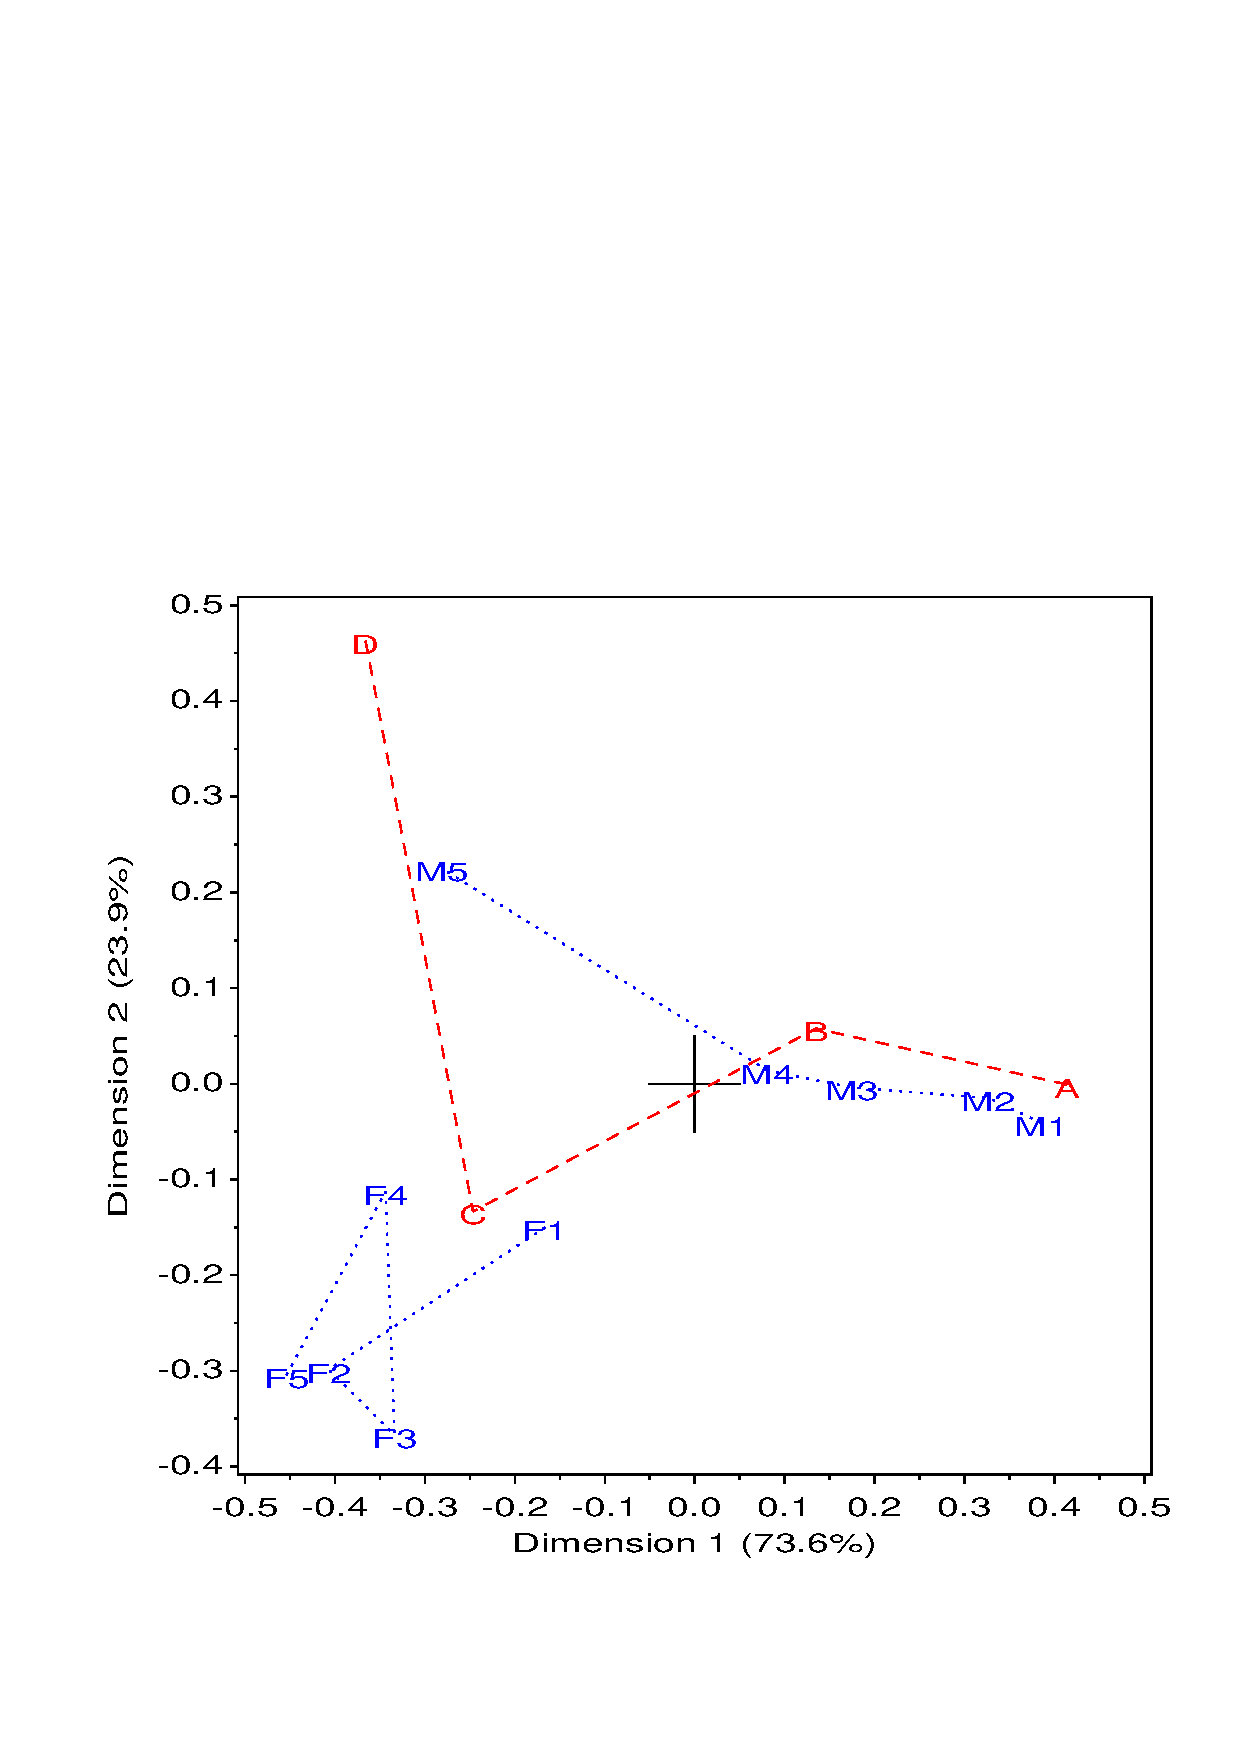
\includegraphics[scale=.6,clip]{vietcores}
  \caption{Correspondence analysis display for model $[SY][R]$}%
  \label{fig:vietcores}
\end{figure}

Both \figref{fig:mosviet} and \figref{fig:vietcores} indicate that our
assumption of linear spacing of year for men is incorrect, particularly
for graduate students.
A simple approach is to replace the variable \pname{year} with a new
variable, \pname{YR}, for which graduate students are some number
greater than 5.
Varying the year for graduate students over the range 5--10 gives
the residual \GSQ\ values (with 21 df)
in \tabref{tab:vietgrad}, and suggests that
7 years for graduate students gives the best fit.  The plot
of fitted and observed values under the revised model is shown in \figref{fig:vietnam3}.
\input{ch7/sas/vietnam3}
\input{ch7/tab/vietgrad}

%% two subfig side-by-side
\begin{figure}[htb]
 \begin{minipage}[t]{.49\linewidth}
  \includegraphics[width=1\linewidth]{vietnam31}
 \end{minipage}%
 \hfill
 \begin{minipage}[t]{.49\linewidth}
  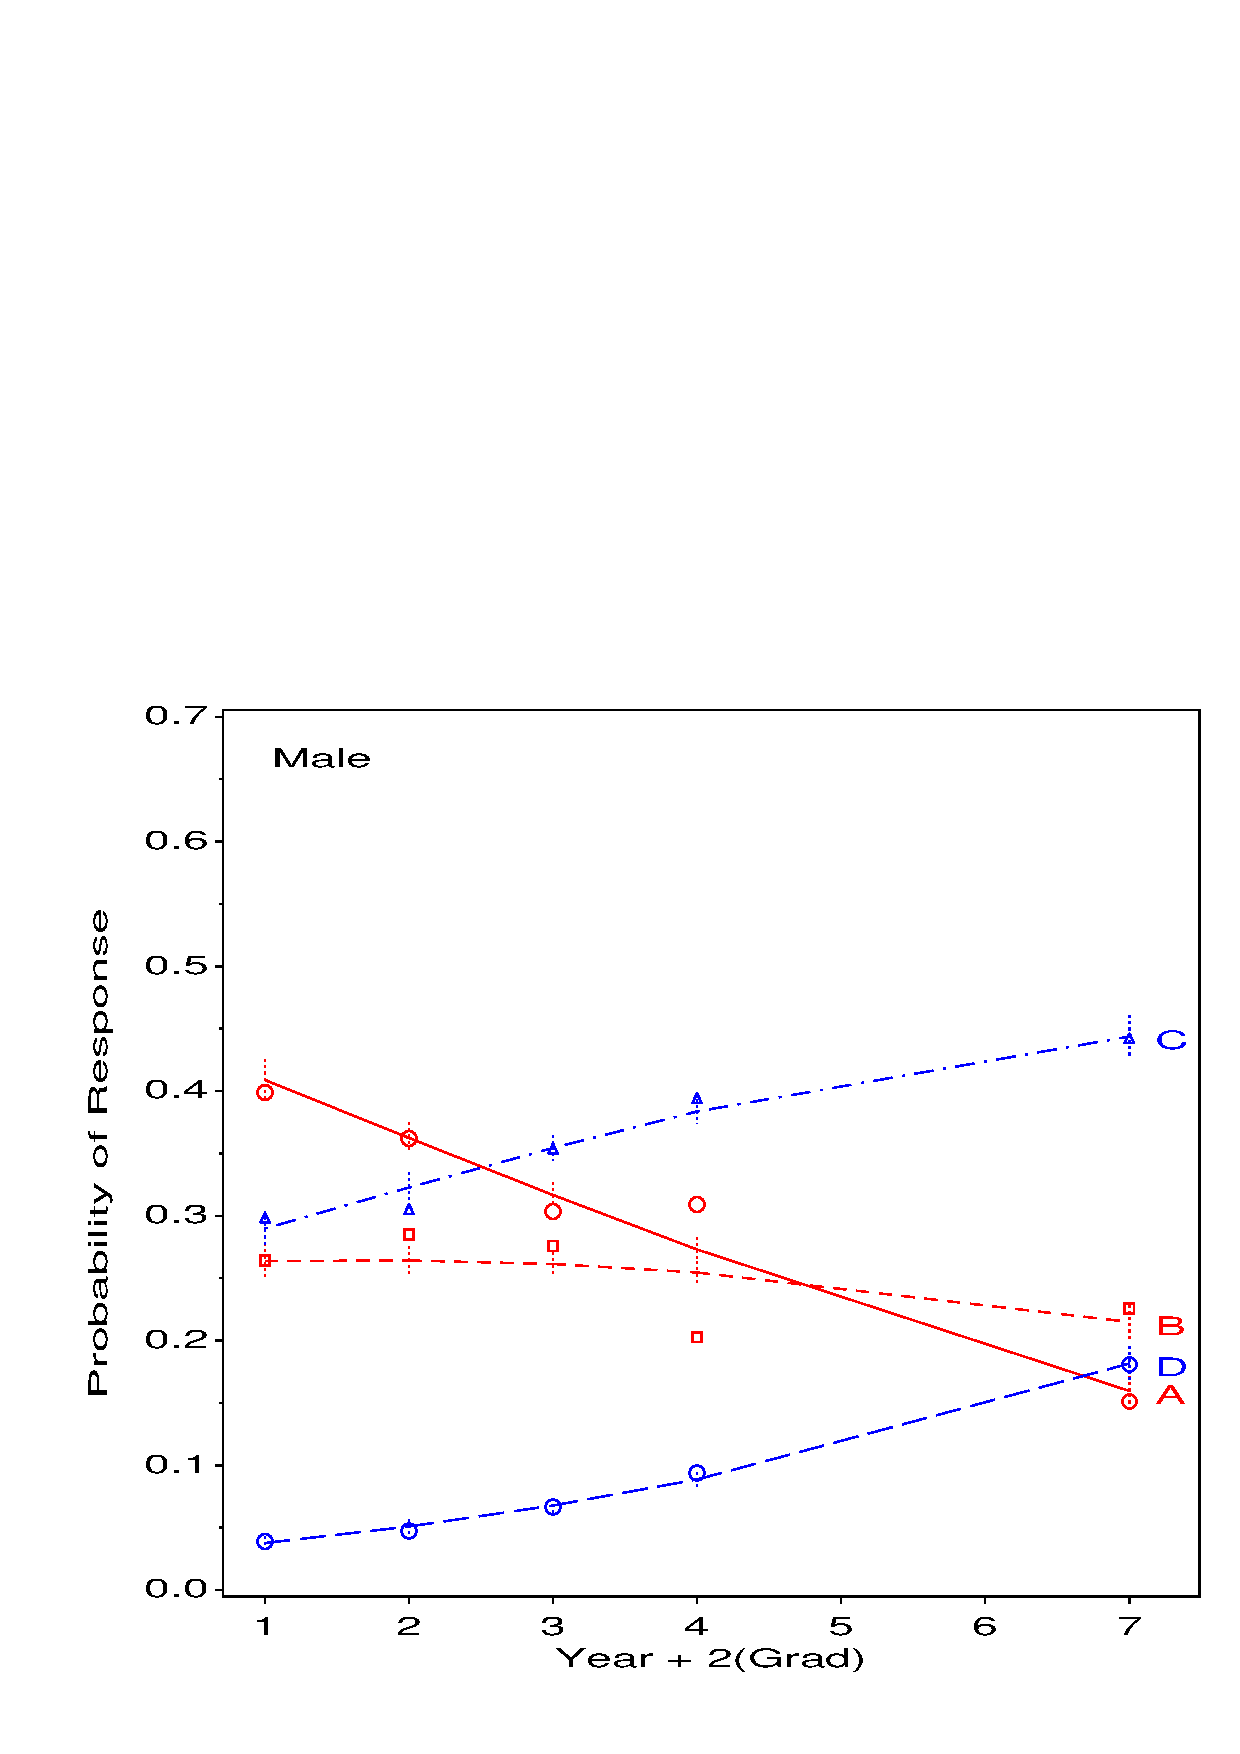
\includegraphics[width=1\linewidth]{vietnam32}
 \end{minipage}
 \caption{Observed and fitted probabilities for model $R = S + Y_{lin}(M)$, Graduate students=7}\label{fig:vietnam3}
\end{figure}

This model fits quite well overall, but there are still several
discrepant points.
We examine residuals and influence diagnostics for this model in
the following section
(\exref{ex:vietnam3}).
\end{Example}


%% two subfig side-by-side
\begin{figure}[htb]
 \begin{minipage}[t]{.49\linewidth}
  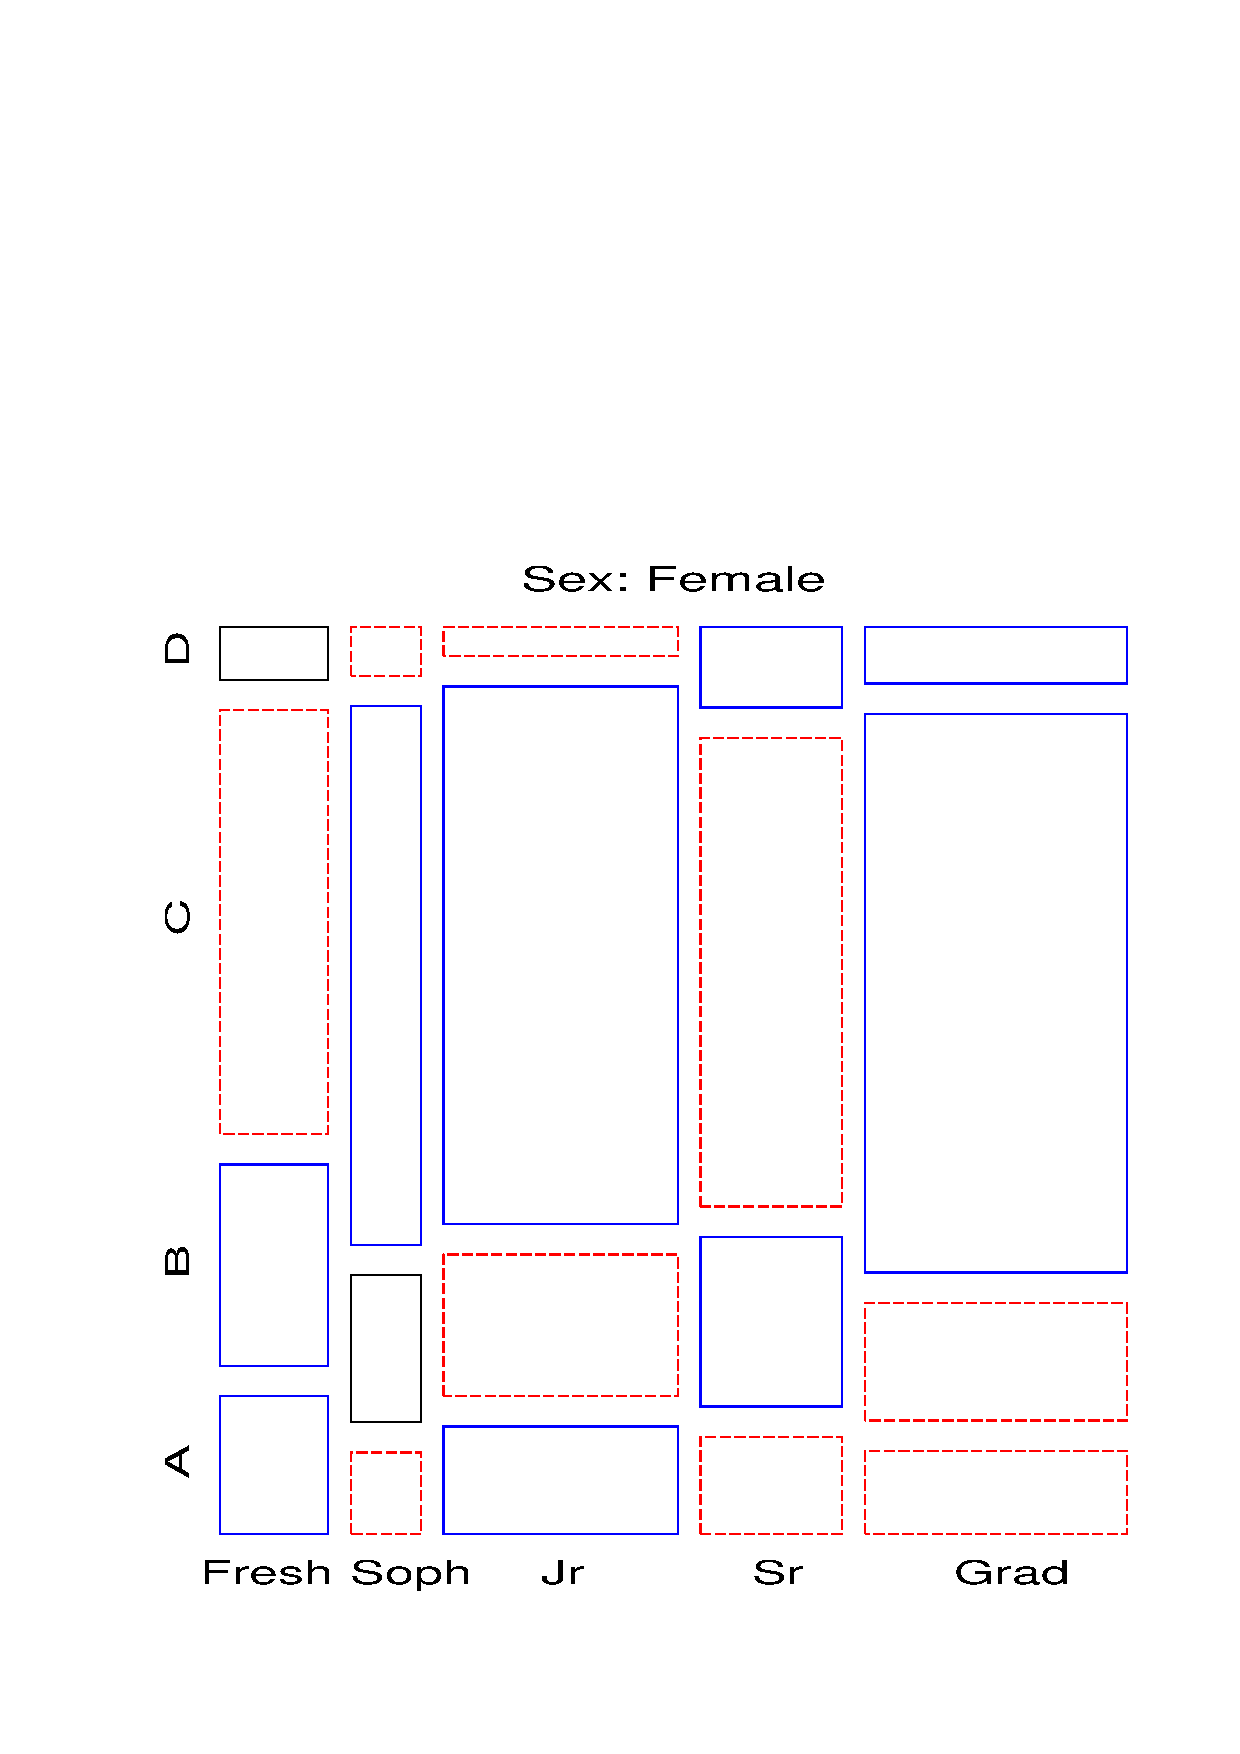
\includegraphics[width=1\linewidth,clip]{mosviet1}
 \end{minipage}%
 \hfill
 \begin{minipage}[t]{.49\linewidth}
  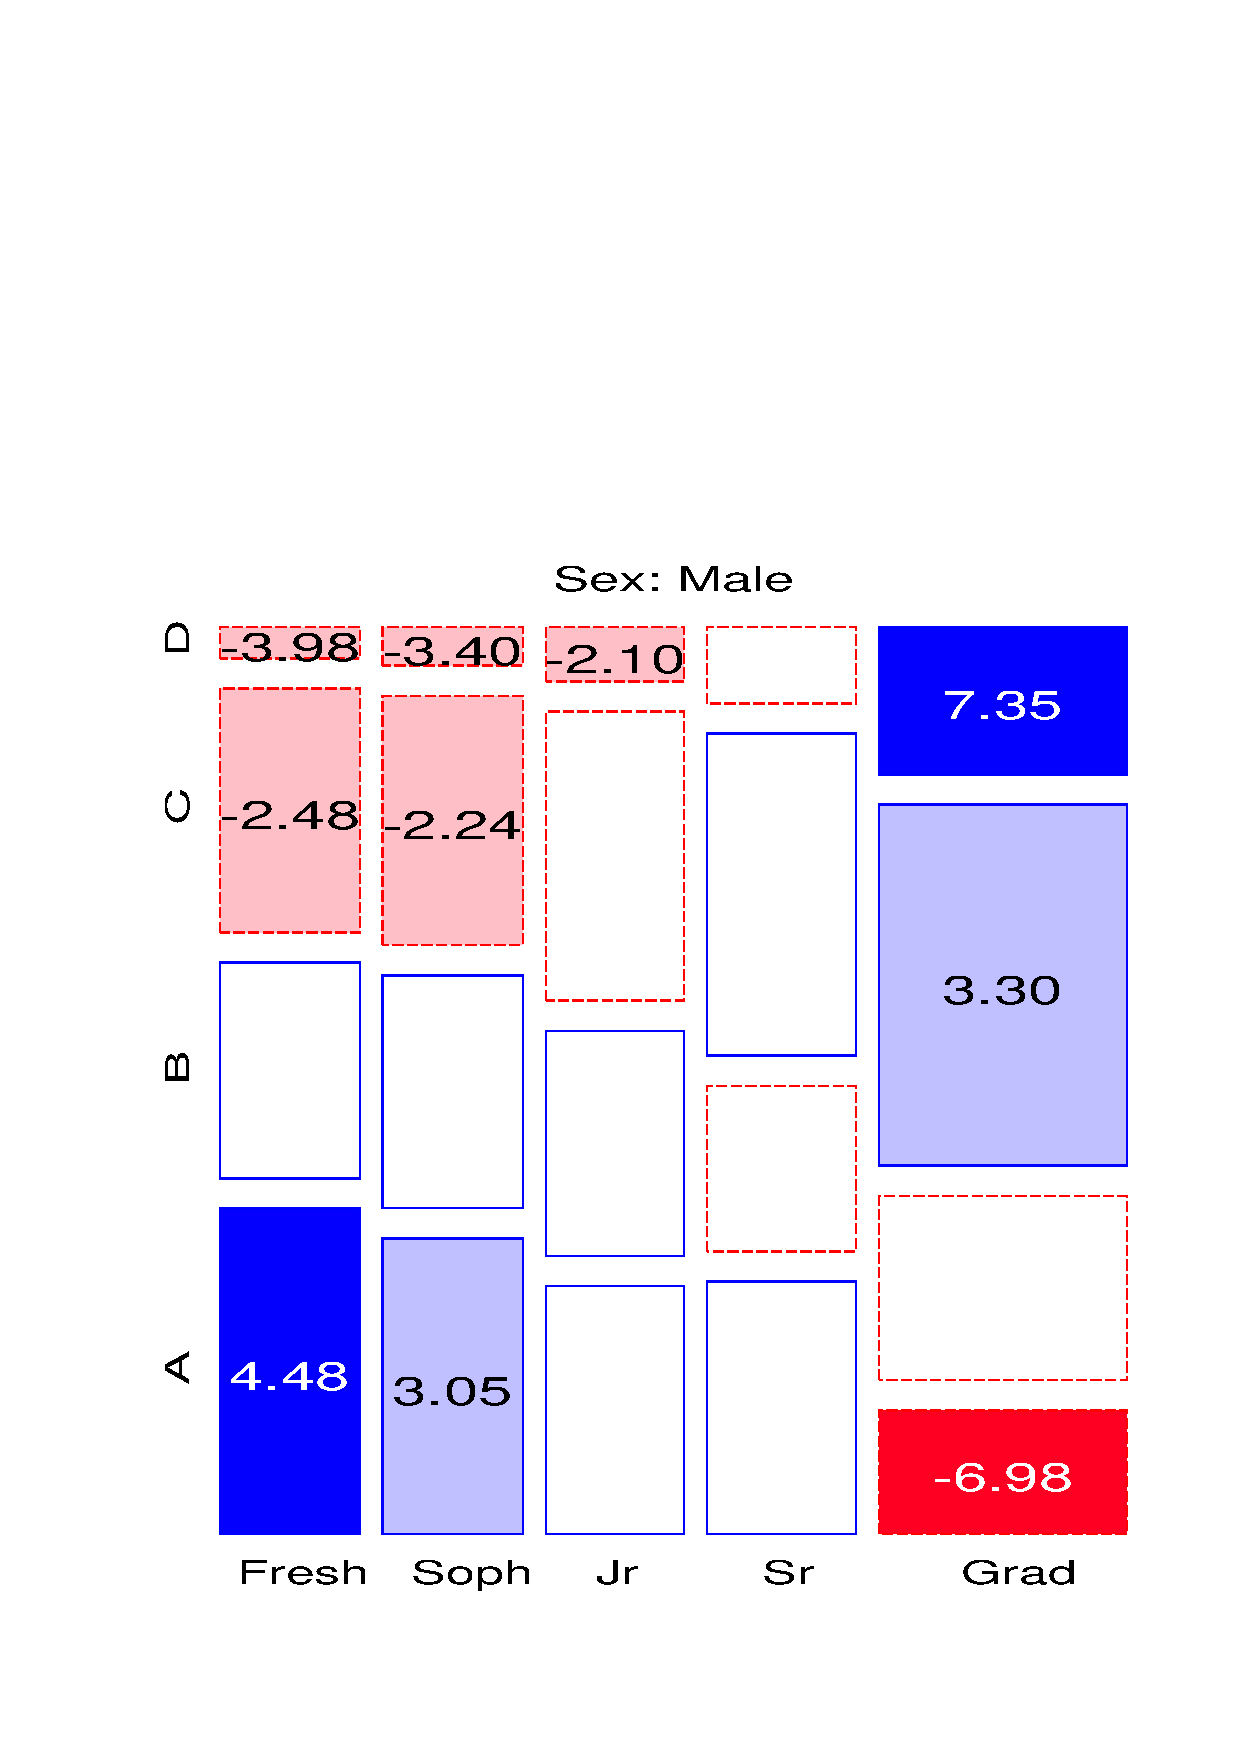
\includegraphics[width=1\linewidth,clip]{mosviet2}
 \end{minipage}
 \caption{Partial mosaic plots, by sex, for Vietnam war data}\label{fig:mosviet}
\end{figure}
With the variables in each mosaic ordered Year, Response,
recall that the height of each bar shows the (conditional) proportion
of students in each year who chose each response. There is no systematic
pattern for women, but the pattern of heights of the boxes, and of the
residuals from independence for men is very systematic.
The trend over years is easiest to see for responses A and D;
note that there is a large jump in proportion choosing these responses
between 4th year students and graduate students.
Perhaps our assumption of a linear trend with year for males needs
adjustment.

A \CA\ plot also displays residuals from a background model.  Here
we choose the null-response model of joint independence, $[SY] [R]$, so that all associations
between the response and the sex-year combinations will be shown.
To do this, we first transpose the data so that the responses
are columns and the sex-year populations are rows.
\begin{listing}
%include catdata(vietnam);

*-- Reshape to two-way table, SexYr x Response;
proc transpose data=vietnam prefix=R out=viet2way;
   var count;
   by sex year;

data viet2way;
   set viet2way;
   rename r1=A r2=B r3=C r4=D;
   sexyr = sex || put(year,1.);
   drop _name_;
proc print;

%corresp(data=viet2way, var=A--D, id=sexyr, interp=none join);
\end{listing}

The plot, shown in \figref{fig:vietcores} is quite revealing.
The response points, A--D
largely define the first dimension,
which accounts for 73.6\% of the association from the null-response model.
The year points for men, M1--M5,
are also ordered along this dimension, but male graduate students are far
from the male undergraduates.
The year points for women are tightly clustered, and aligned closest to
response C, their most preferred alternative.
The second dimension seems largely to do with the contrast between the relatively high choice for response D (``immediate withdrawal'')
among male graduate students and general preference for response C
(``de-escalate'') among most women.

%% one figure
\begin{figure}[htb]
  \centering
  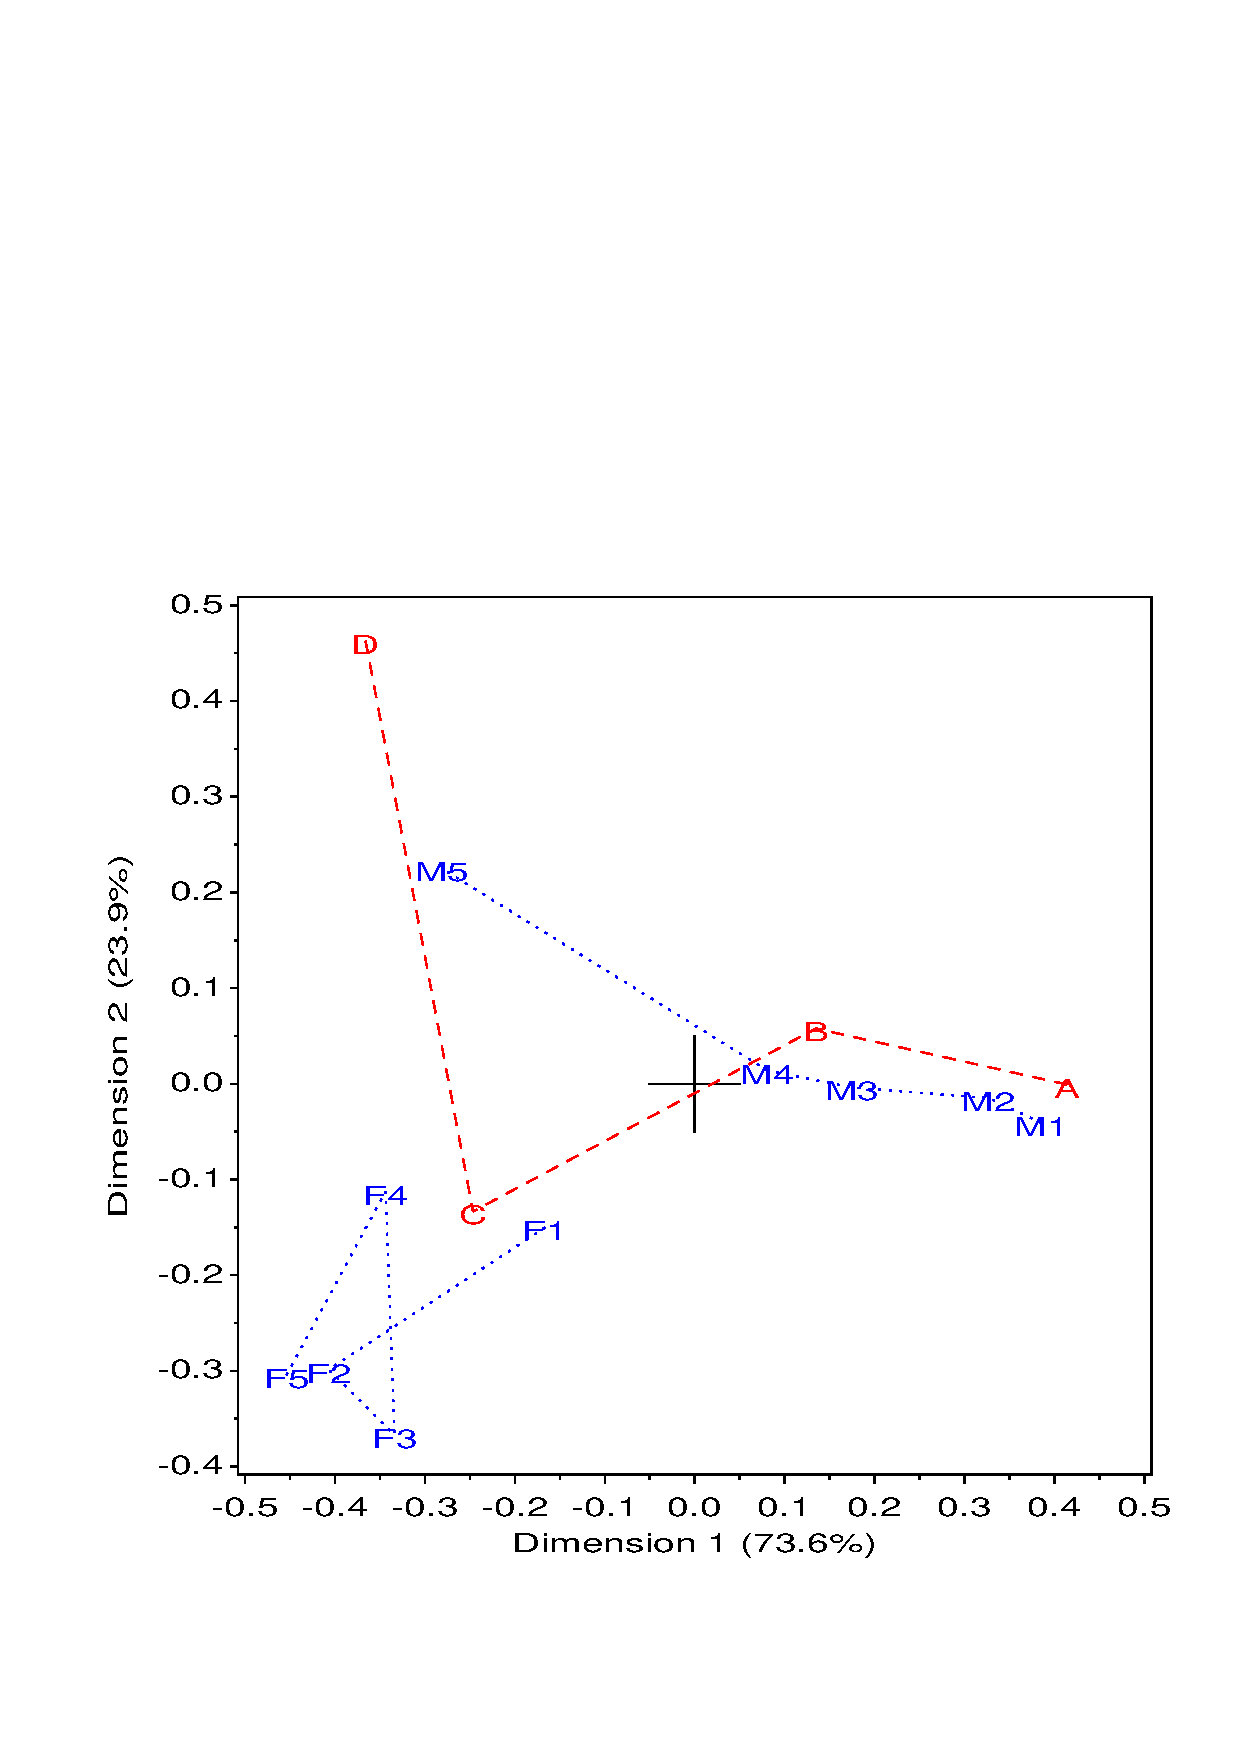
\includegraphics[scale=.6,clip]{vietcores}
  \caption{Correspondence analysis display for model $[SY][R]$}%
  \label{fig:vietcores}
\end{figure}

Both \figref{fig:mosviet} and \figref{fig:vietcores} indicate that our
assumption of linear spacing of year for men is incorrect, particularly
for graduate students.
A simple approach is to replace the variable \pname{year} with a new
variable, \pname{YR}, for which graduate students are some number
greater than 5.
Varying the year for graduate students over the range 5--10 gives
the residual \GSQ\ values (with 21 df)
in \tabref{tab:vietgrad}, and suggests that
7 years for graduate students gives the best fit.  The plot
of fitted and observed values under the revised model is shown in \figref{fig:vietnam3}.
\begin{Example}[vietnam3]{Student opinion about the Vietnam war}
The revised model, with linear effects of year on each logit,
and with graduate students treated as \pname{yr=7}
 shown in \figref{fig:vietnam3} was fit using
\PROC{CATMOD}.  However, influence diagnostics are
easier to obtain using
\PROC{GENMOD}.
The same model can be fit using \PROC{GENMOD} by defining a dummy variable
for women and an interaction between \pname{yr} and a dummy variable
for men.
\begin{listing}
data vietnam;
   set vietnam;
   yr = year + 2*(year=5);
   mlin =  yr * (sex='M');
   female = (sex='F');
   cell = trim(sex)|| put(year,1.)|| trim(put(response,letter.));
   label yr="Year + 2(Grad)";

proc genmod data=vietnam;
   class year sex response;
   model count = year|sex response|mlin  response|female /
         dist=poisson obstats residuals;
   make 'obstats' out=obstats;
\end{listing}
Normally, one would need to merge the input \Dset\ with the \pname{obstats},
and calculate hat values, Cook's D or other quantities for plotting:
\begin{listing}
%let k=8;
data obstats;
   merge vietnam obstats;
   h = hesswgt * std**2;
   cookd = streschi**2 * h/((1-h) * &k);
\end{listing}
where \pname{k=8} is the number of estimated parameters.

Instead, the \macro{INFLGLIM} (\macref{mac:inflglim}) automates these steps, and
gives various influence plots of residuals from a given
model.  The macro plots all combinations of the variables given
by the \mparm{GY}{INFLGLIM} against the variables given by the \mparm{GX}{INFLGLIM},
using a bubble symbol whose size is proportional to the
\mparm{BUBBLE}{INFLGLIM}, usually Cook's D.

Here, we plot the one-step estimates of change in deviance
($\Delta G_{(-i)}^2$, or \pname{DIFDEV})
due to deleting each cell against hat values,
using bubble symbols with area proportional to Cook's D.
The \mparm{infl}{INFLGLIM} determines the criterion for labeling
potentially influential points.
\begin{listing}
%inflglim(data=vietnam, resp=count,
    class=year sex response,
    model= year|sex  response|mlin  response|female,
    dist=poisson, id=cell,
    infl=%str(difdev>4 or &bubble>1 or hat>1.5*&hcrit),
    gy=difdev, gx=hat, bubble=cookd);
\end{listing}

This plot (\figref{fig:vietgen3}) shows that there are still two
large residuals: 4th year men choose response B substantially less often
than predicted (accounting for over one-third of the model deviance), and first year women choose response C less than
predicted.
%% one figure
\begin{figure}[htb]
  \centering
  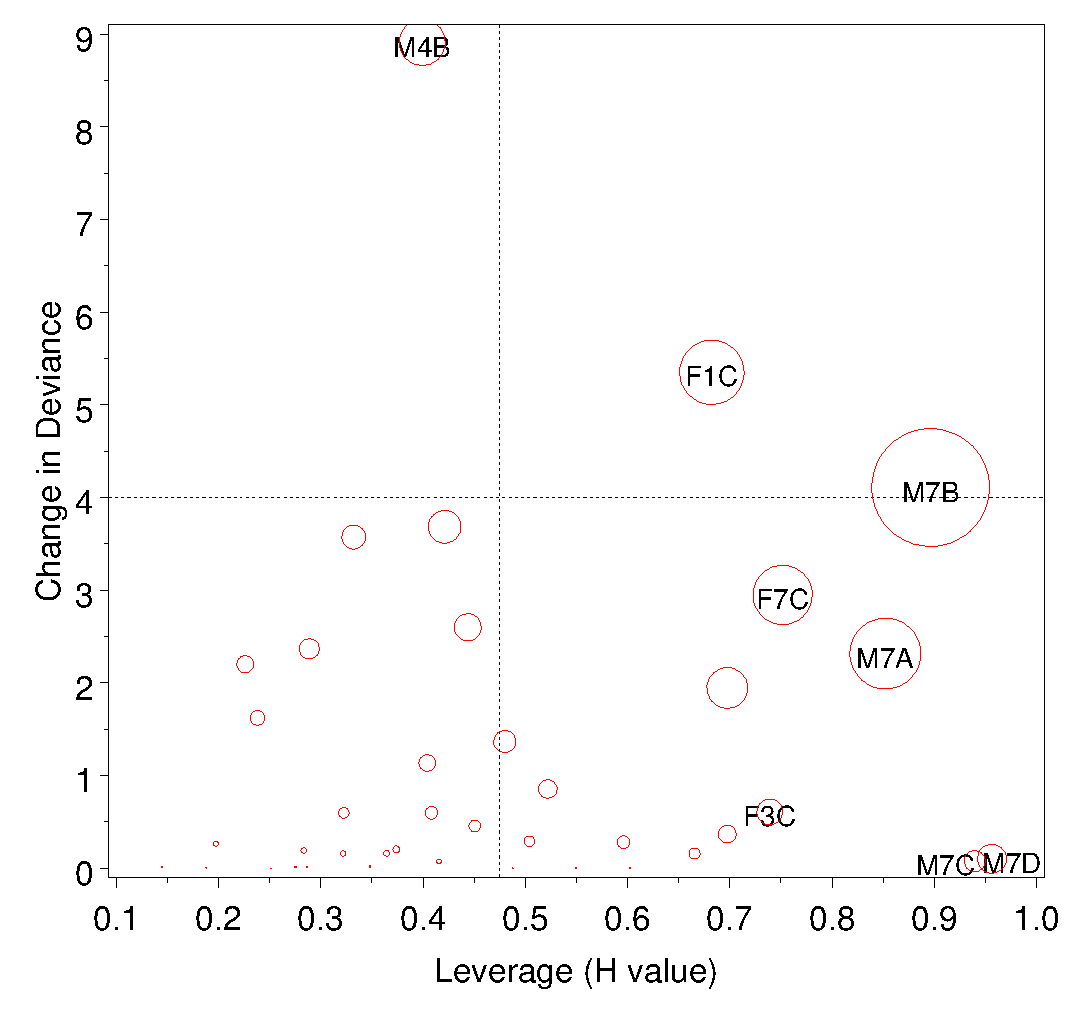
\includegraphics[scale=.6]{vietgen3}
  \caption{Influence plot for model $R = S + Y_{lin}(M)$, Graduate students=7}%
  \label{fig:vietgen3}
\end{figure}
We complete the analysis and this example with a half-normal plot of
these residuals, shown in \figref{fig:vietgen4}.  Although there is
evidence of non-normality in the distribution of residuals,  even the largest
values are within the simulated envelope.
\begin{listing}
%halfnorm(data=vietnam, resp=count,
   class=sex year response,
   model=year|sex  response|mlin  response|female,
   dist=poisson, id=cell);
\end{listing}

\begin{figure}[htb]
  \centering
  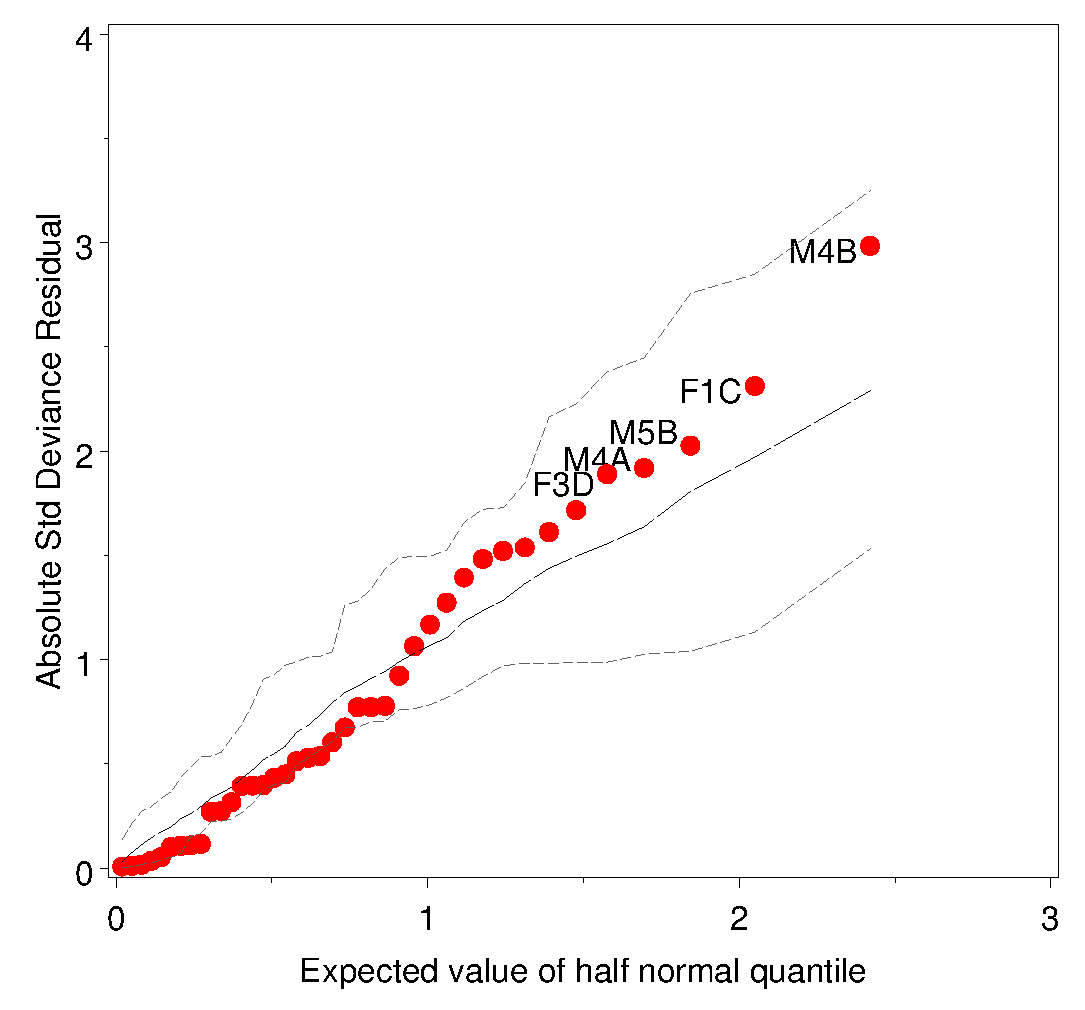
\includegraphics[scale=.6]{vietgen4}
  \caption{Half-normal plot for model $R = S + Y_{lin}(M)$, Graduate students=7}%
  \label{fig:vietgen4}
\end{figure}
\end{Example}

\begin{table}[htb]
 \caption{Profile deviance analysis of Year for Graduate Students}\label{tab:vietgrad}
 \begin{center}
 \begin{tabular}{cr}
  \hline
  Grad Year & \GSQ (21) \\
  \hline
  5 &  38.10 \\ 
  6 &  26.69 \\ 
  7 &  23.87 \\ 
  8 &  23.99 \\ 
  9 &  25.13 \\ 
  10 & 26.58 \\ 
  \hline
 \end{tabular}
 \end{center}
\end{table}


%% two subfig side-by-side
\begin{figure}[htb]
 \begin{minipage}[t]{.49\linewidth}
  \includegraphics[width=1\linewidth]{vietnam31}
 \end{minipage}%
 \hfill
 \begin{minipage}[t]{.49\linewidth}
  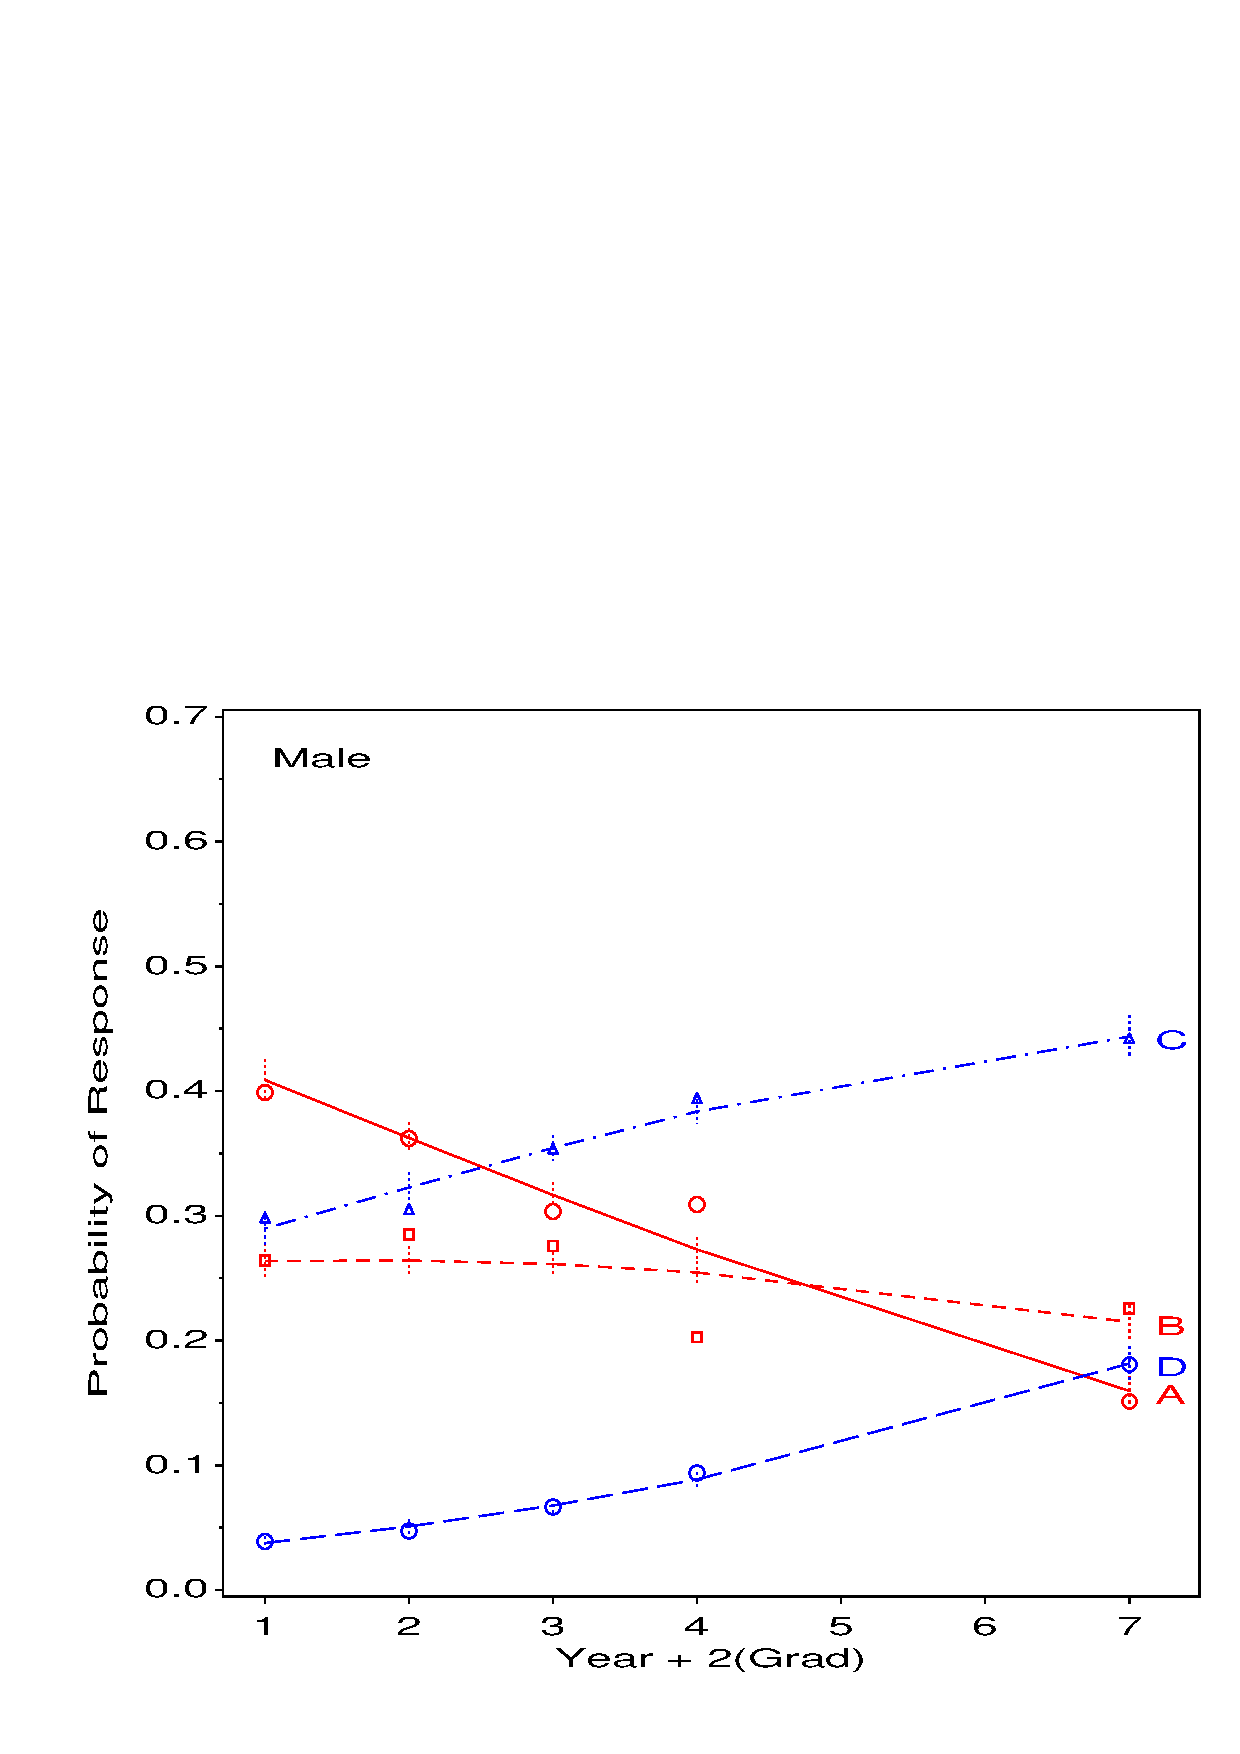
\includegraphics[width=1\linewidth]{vietnam32}
 \end{minipage}
 \caption{Observed and fitted probabilities for model $R = S + Y_{lin}(M)$, Graduate students=7}\label{fig:vietnam3}
\end{figure}

This model fits quite well overall, but there are still several
discrepant points.
We examine residuals and influence diagnostics for this model in
the following section
(\exref{ex:vietnam3}).
\end{Example}


%% two subfig side-by-side
\begin{figure}[htb]
 \begin{minipage}[t]{.49\linewidth}
  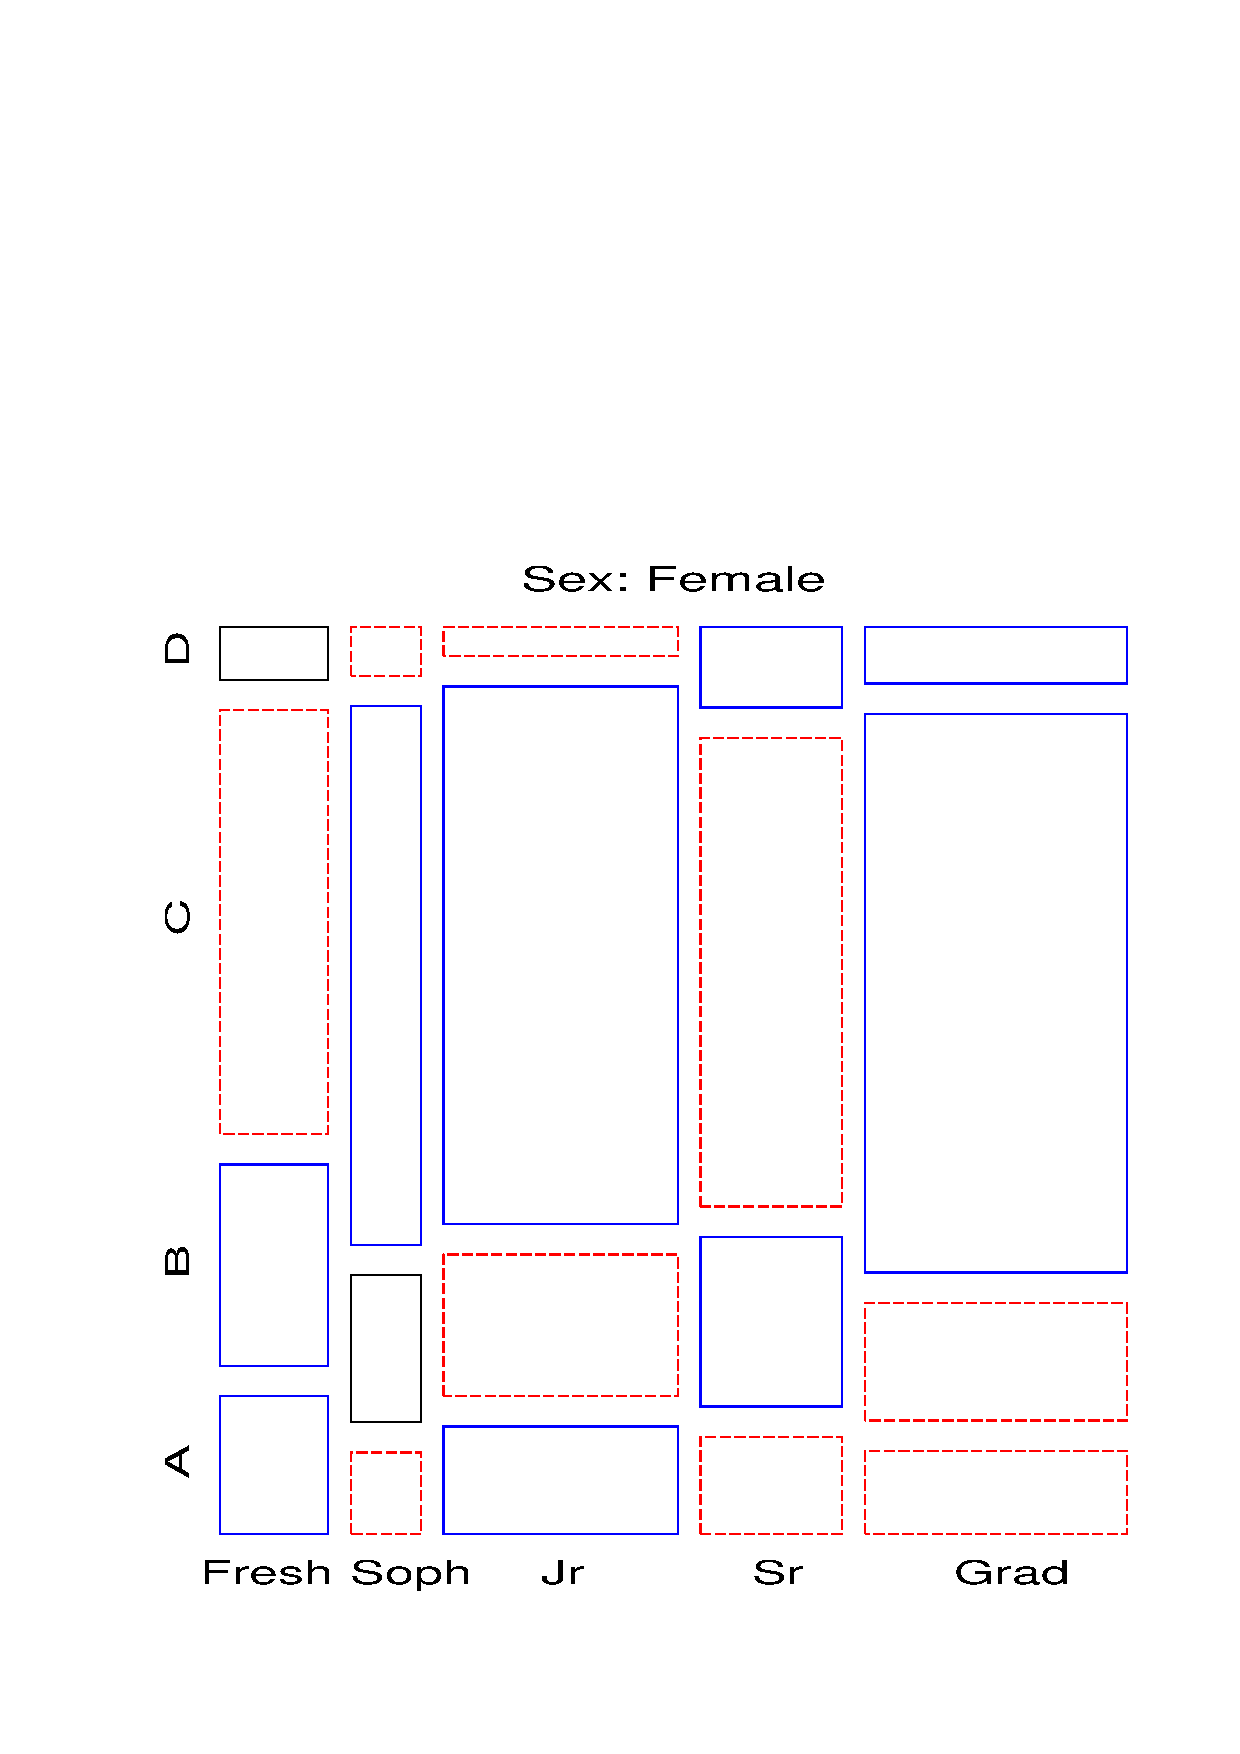
\includegraphics[width=1\linewidth,clip]{mosviet1}
 \end{minipage}%
 \hfill
 \begin{minipage}[t]{.49\linewidth}
  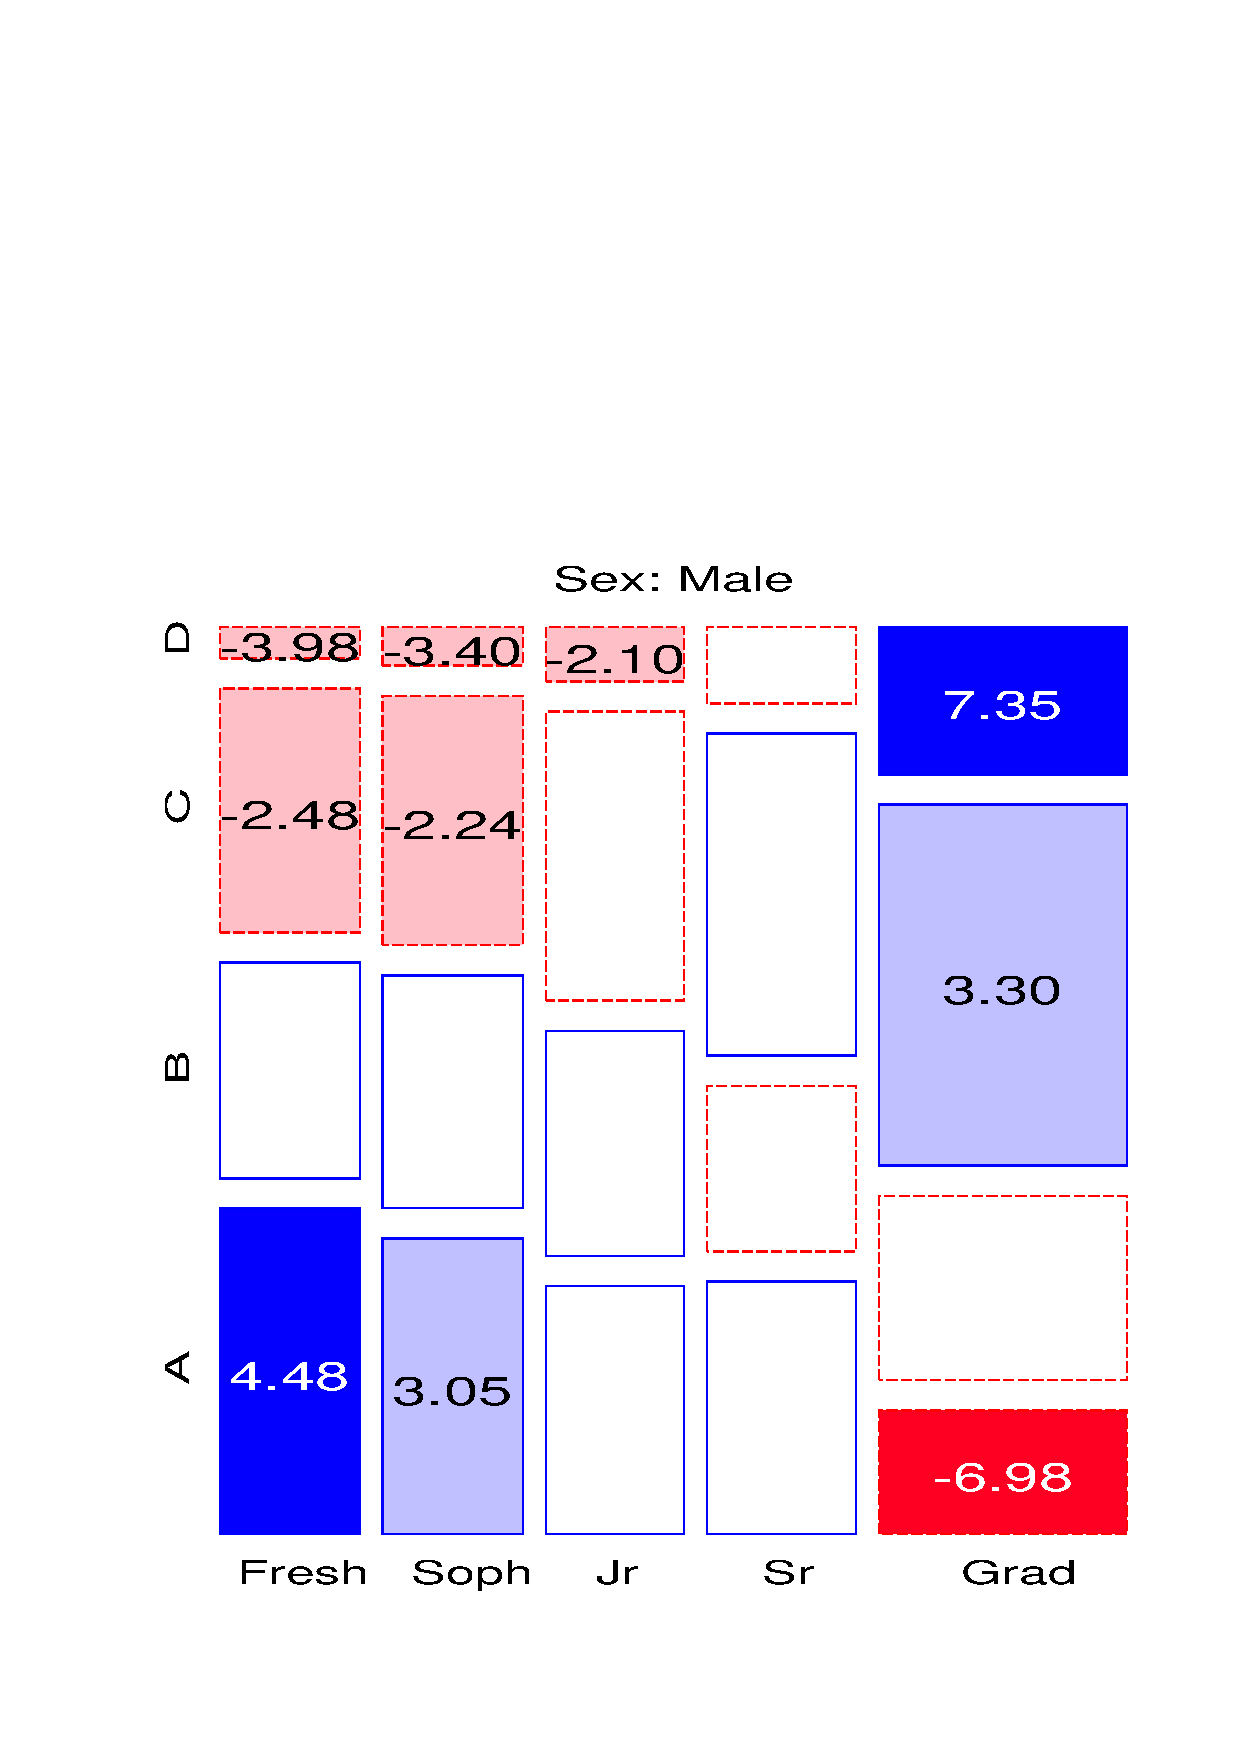
\includegraphics[width=1\linewidth,clip]{mosviet2}
 \end{minipage}
 \caption{Partial mosaic plots, by sex, for Vietnam war data}\label{fig:mosviet}
\end{figure}
With the variables in each mosaic ordered Year, Response,
recall that the height of each bar shows the (conditional) proportion
of students in each year who chose each response. There is no systematic
pattern for women, but the pattern of heights of the boxes, and of the
residuals from independence for men is very systematic.
The trend over years is easiest to see for responses A and D;
note that there is a large jump in proportion choosing these responses
between 4th year students and graduate students.
Perhaps our assumption of a linear trend with year for males needs
adjustment.

A \CA\ plot also displays residuals from a background model.  Here
we choose the null-response model of joint independence, $[SY] [R]$, so that all associations
between the response and the sex-year combinations will be shown.
To do this, we first transpose the data so that the responses
are columns and the sex-year populations are rows.
\begin{listing}
%include catdata(vietnam);

*-- Reshape to two-way table, SexYr x Response;
proc transpose data=vietnam prefix=R out=viet2way;
   var count;
   by sex year;

data viet2way;
   set viet2way;
   rename r1=A r2=B r3=C r4=D;
   sexyr = sex || put(year,1.);
   drop _name_;
proc print;

%corresp(data=viet2way, var=A--D, id=sexyr, interp=none join);
\end{listing}

The plot, shown in \figref{fig:vietcores} is quite revealing.
The response points, A--D
largely define the first dimension,
which accounts for 73.6\% of the association from the null-response model.
The year points for men, M1--M5,
are also ordered along this dimension, but male graduate students are far
from the male undergraduates.
The year points for women are tightly clustered, and aligned closest to
response C, their most preferred alternative.
The second dimension seems largely to do with the contrast between the relatively high choice for response D (``immediate withdrawal'')
among male graduate students and general preference for response C
(``de-escalate'') among most women.

%% one figure
\begin{figure}[htb]
  \centering
  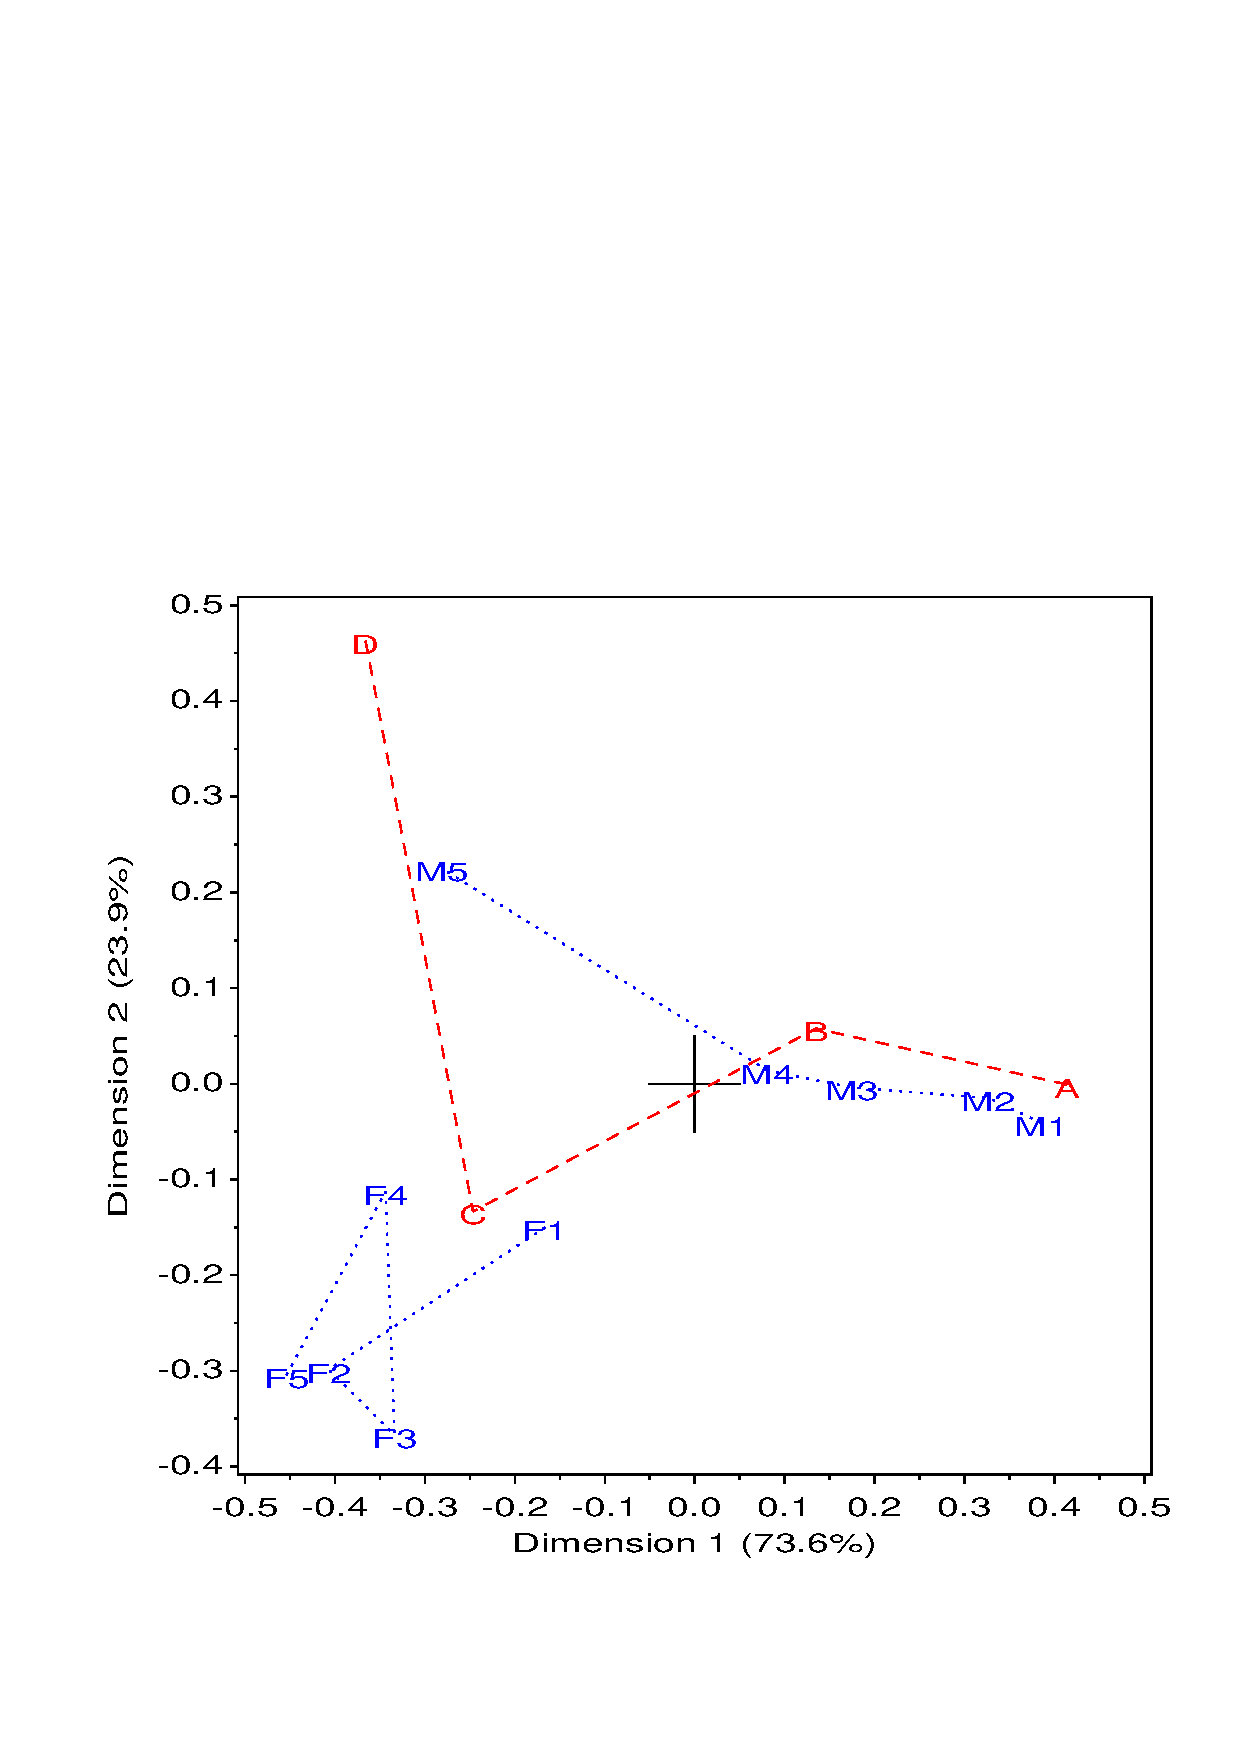
\includegraphics[scale=.6,clip]{vietcores}
  \caption{Correspondence analysis display for model $[SY][R]$}%
  \label{fig:vietcores}
\end{figure}

Both \figref{fig:mosviet} and \figref{fig:vietcores} indicate that our
assumption of linear spacing of year for men is incorrect, particularly
for graduate students.
A simple approach is to replace the variable \pname{year} with a new
variable, \pname{YR}, for which graduate students are some number
greater than 5.
Varying the year for graduate students over the range 5--10 gives
the residual \GSQ\ values (with 21 df)
in \tabref{tab:vietgrad}, and suggests that
7 years for graduate students gives the best fit.  The plot
of fitted and observed values under the revised model is shown in \figref{fig:vietnam3}.
\begin{Example}[vietnam3]{Student opinion about the Vietnam war}
The revised model, with linear effects of year on each logit,
and with graduate students treated as \pname{yr=7}
 shown in \figref{fig:vietnam3} was fit using
\PROC{CATMOD}.  However, influence diagnostics are
easier to obtain using
\PROC{GENMOD}.
The same model can be fit using \PROC{GENMOD} by defining a dummy variable
for women and an interaction between \pname{yr} and a dummy variable
for men.
\begin{listing}
data vietnam;
   set vietnam;
   yr = year + 2*(year=5);
   mlin =  yr * (sex='M');
   female = (sex='F');
   cell = trim(sex)|| put(year,1.)|| trim(put(response,letter.));
   label yr="Year + 2(Grad)";

proc genmod data=vietnam;
   class year sex response;
   model count = year|sex response|mlin  response|female /
         dist=poisson obstats residuals;
   make 'obstats' out=obstats;
\end{listing}
Normally, one would need to merge the input \Dset\ with the \pname{obstats},
and calculate hat values, Cook's D or other quantities for plotting:
\begin{listing}
%let k=8;
data obstats;
   merge vietnam obstats;
   h = hesswgt * std**2;
   cookd = streschi**2 * h/((1-h) * &k);
\end{listing}
where \pname{k=8} is the number of estimated parameters.

Instead, the \macro{INFLGLIM} (\macref{mac:inflglim}) automates these steps, and
gives various influence plots of residuals from a given
model.  The macro plots all combinations of the variables given
by the \mparm{GY}{INFLGLIM} against the variables given by the \mparm{GX}{INFLGLIM},
using a bubble symbol whose size is proportional to the
\mparm{BUBBLE}{INFLGLIM}, usually Cook's D.

Here, we plot the one-step estimates of change in deviance
($\Delta G_{(-i)}^2$, or \pname{DIFDEV})
due to deleting each cell against hat values,
using bubble symbols with area proportional to Cook's D.
The \mparm{infl}{INFLGLIM} determines the criterion for labeling
potentially influential points.
\begin{listing}
%inflglim(data=vietnam, resp=count,
    class=year sex response,
    model= year|sex  response|mlin  response|female,
    dist=poisson, id=cell,
    infl=%str(difdev>4 or &bubble>1 or hat>1.5*&hcrit),
    gy=difdev, gx=hat, bubble=cookd);
\end{listing}

This plot (\figref{fig:vietgen3}) shows that there are still two
large residuals: 4th year men choose response B substantially less often
than predicted (accounting for over one-third of the model deviance), and first year women choose response C less than
predicted.
%% one figure
\begin{figure}[htb]
  \centering
  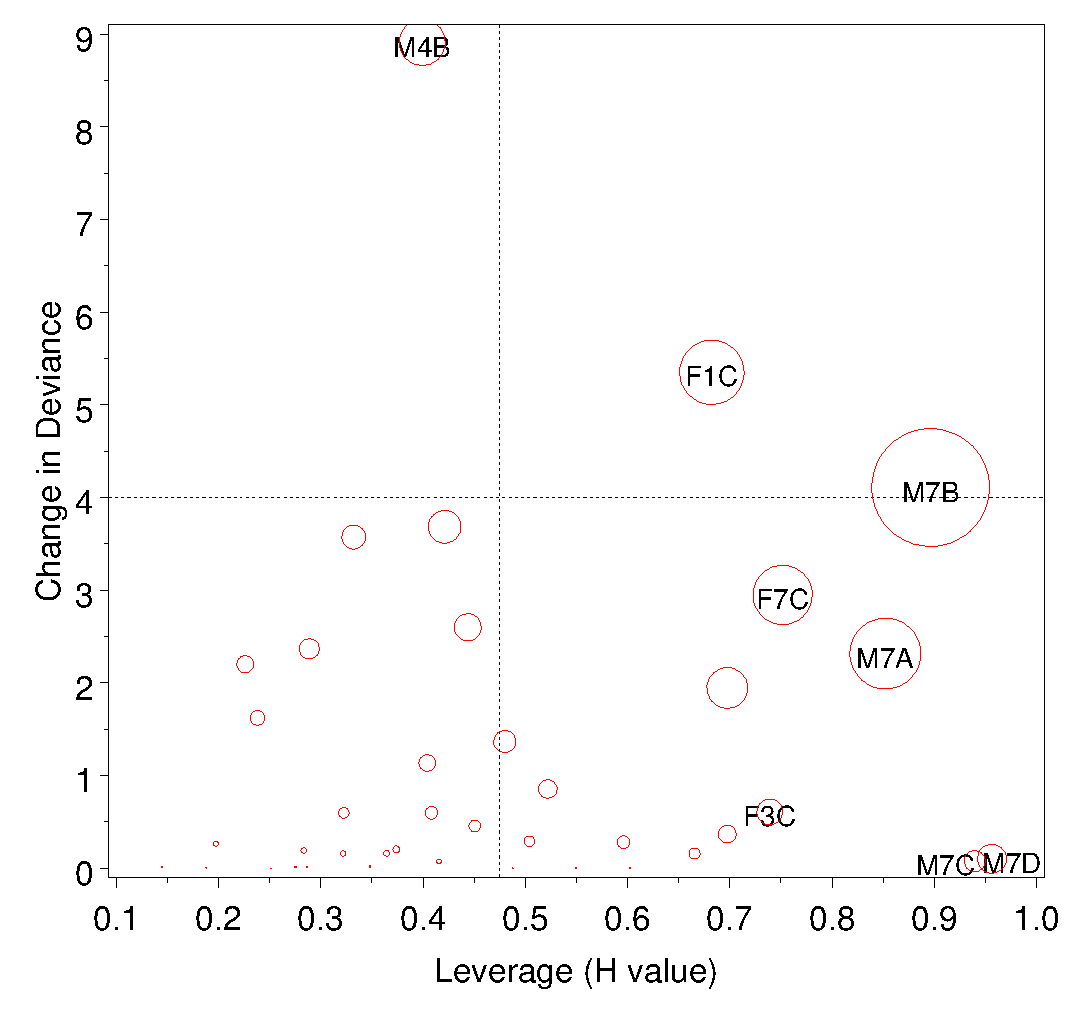
\includegraphics[scale=.6]{vietgen3}
  \caption{Influence plot for model $R = S + Y_{lin}(M)$, Graduate students=7}%
  \label{fig:vietgen3}
\end{figure}
We complete the analysis and this example with a half-normal plot of
these residuals, shown in \figref{fig:vietgen4}.  Although there is
evidence of non-normality in the distribution of residuals,  even the largest
values are within the simulated envelope.
\begin{listing}
%halfnorm(data=vietnam, resp=count,
   class=sex year response,
   model=year|sex  response|mlin  response|female,
   dist=poisson, id=cell);
\end{listing}

\begin{figure}[htb]
  \centering
  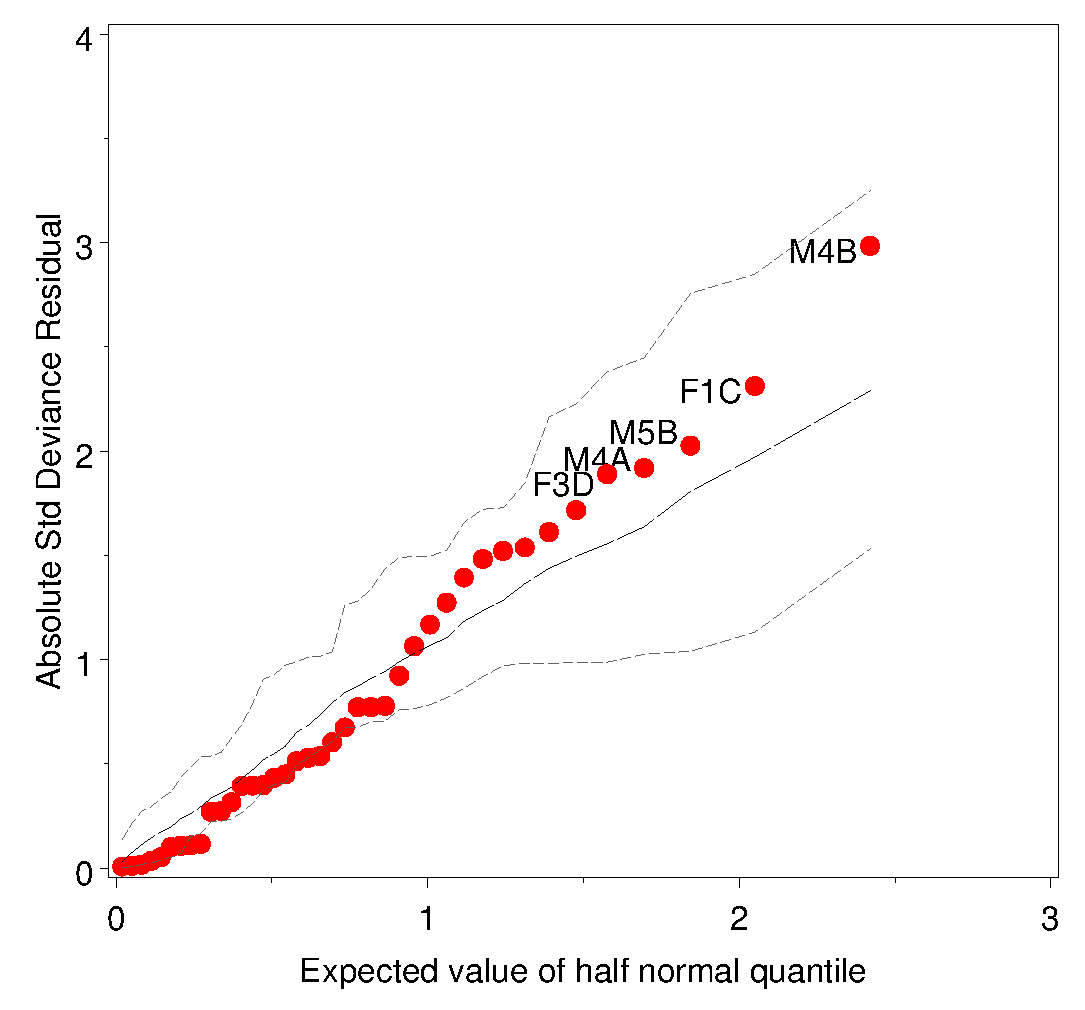
\includegraphics[scale=.6]{vietgen4}
  \caption{Half-normal plot for model $R = S + Y_{lin}(M)$, Graduate students=7}%
  \label{fig:vietgen4}
\end{figure}
\end{Example}

\begin{table}[htb]
 \caption{Profile deviance analysis of Year for Graduate Students}\label{tab:vietgrad}
 \begin{center}
 \begin{tabular}{cr}
  \hline
  Grad Year & \GSQ (21) \\
  \hline
  5 &  38.10 \\ 
  6 &  26.69 \\ 
  7 &  23.87 \\ 
  8 &  23.99 \\ 
  9 &  25.13 \\ 
  10 & 26.58 \\ 
  \hline
 \end{tabular}
 \end{center}
\end{table}


%% two subfig side-by-side
\begin{figure}[htb]
 \begin{minipage}[t]{.49\linewidth}
  \includegraphics[width=1\linewidth]{vietnam31}
 \end{minipage}%
 \hfill
 \begin{minipage}[t]{.49\linewidth}
  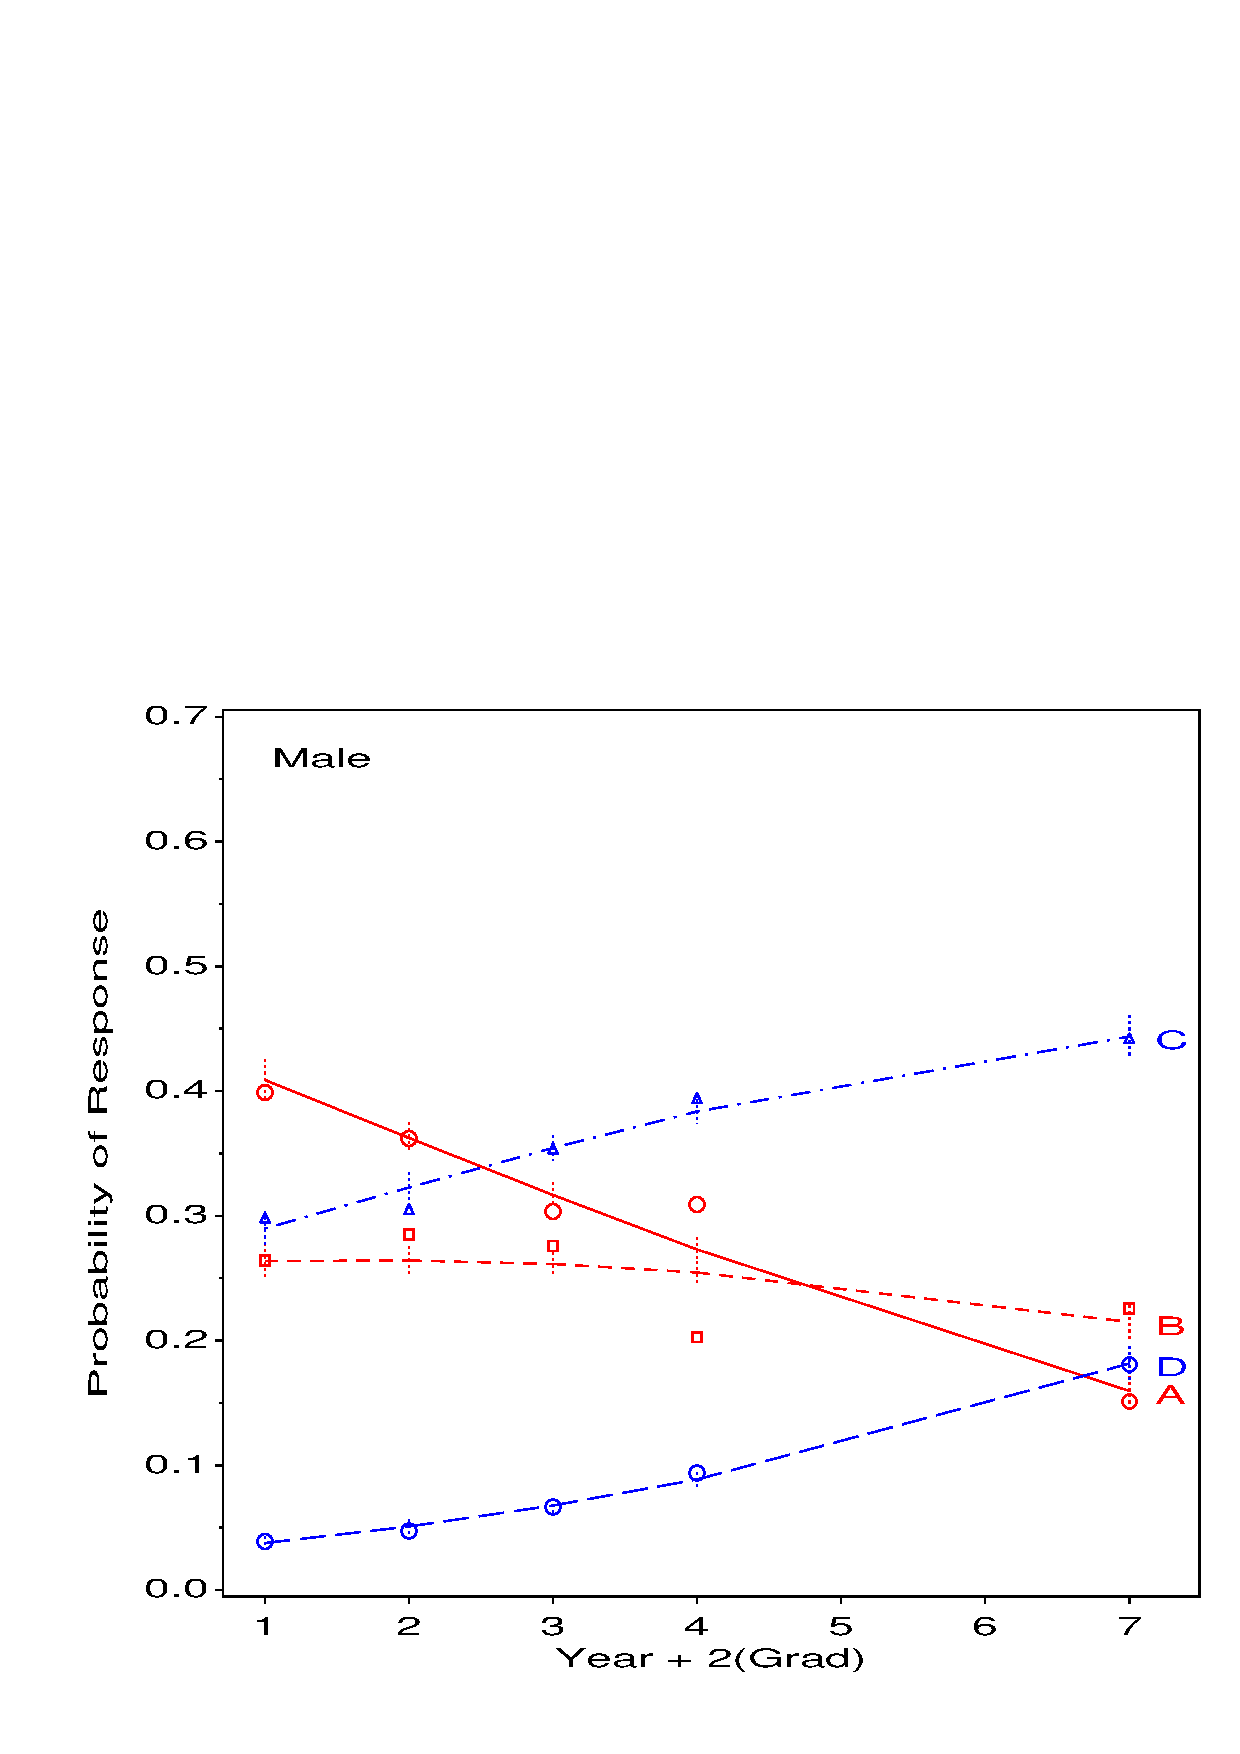
\includegraphics[width=1\linewidth]{vietnam32}
 \end{minipage}
 \caption{Observed and fitted probabilities for model $R = S + Y_{lin}(M)$, Graduate students=7}\label{fig:vietnam3}
\end{figure}

This model fits quite well overall, but there are still several
discrepant points.
We examine residuals and influence diagnostics for this model in
the following section
(\exref{ex:vietnam3}).
\end{Example}


%% two subfig side-by-side
\begin{figure}[htb]
 \begin{minipage}[t]{.49\linewidth}
  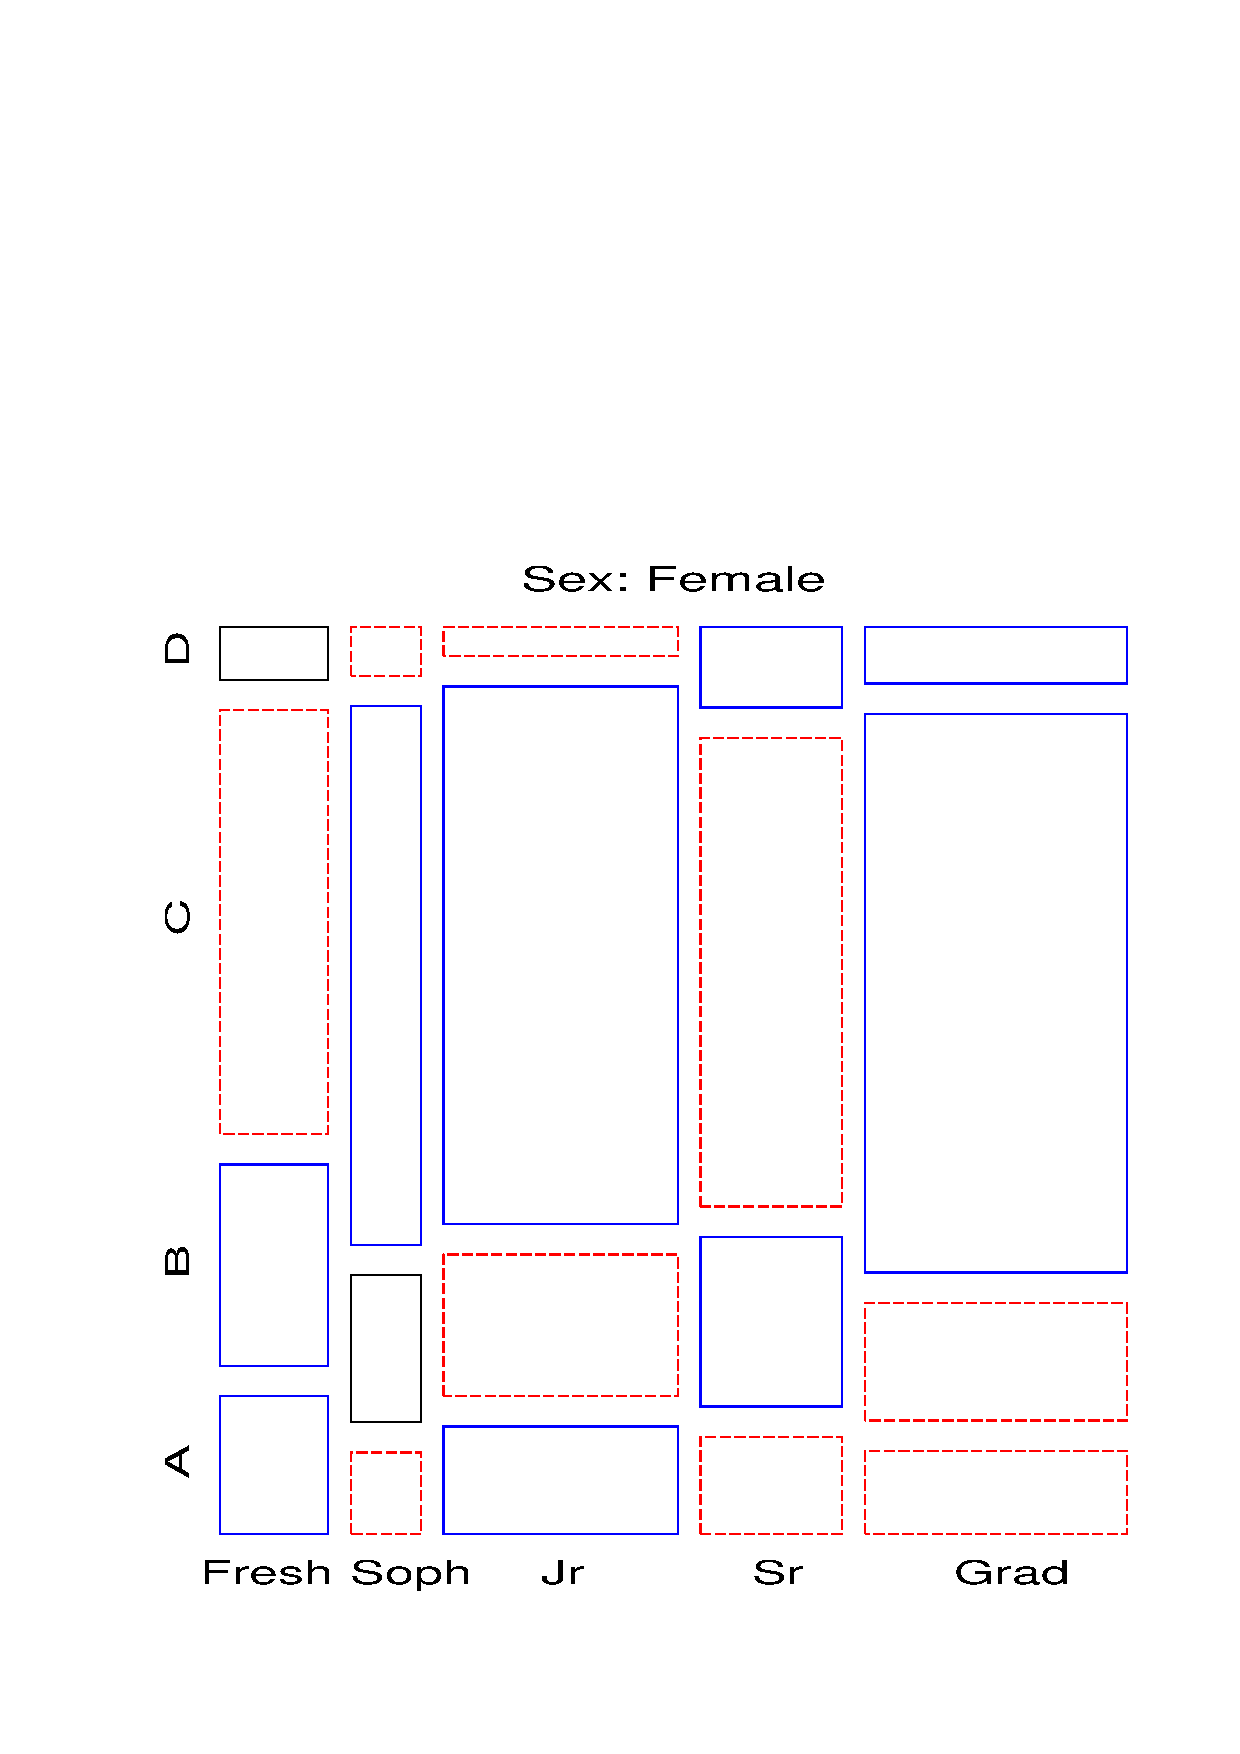
\includegraphics[width=1\linewidth,clip]{mosviet1}
 \end{minipage}%
 \hfill
 \begin{minipage}[t]{.49\linewidth}
  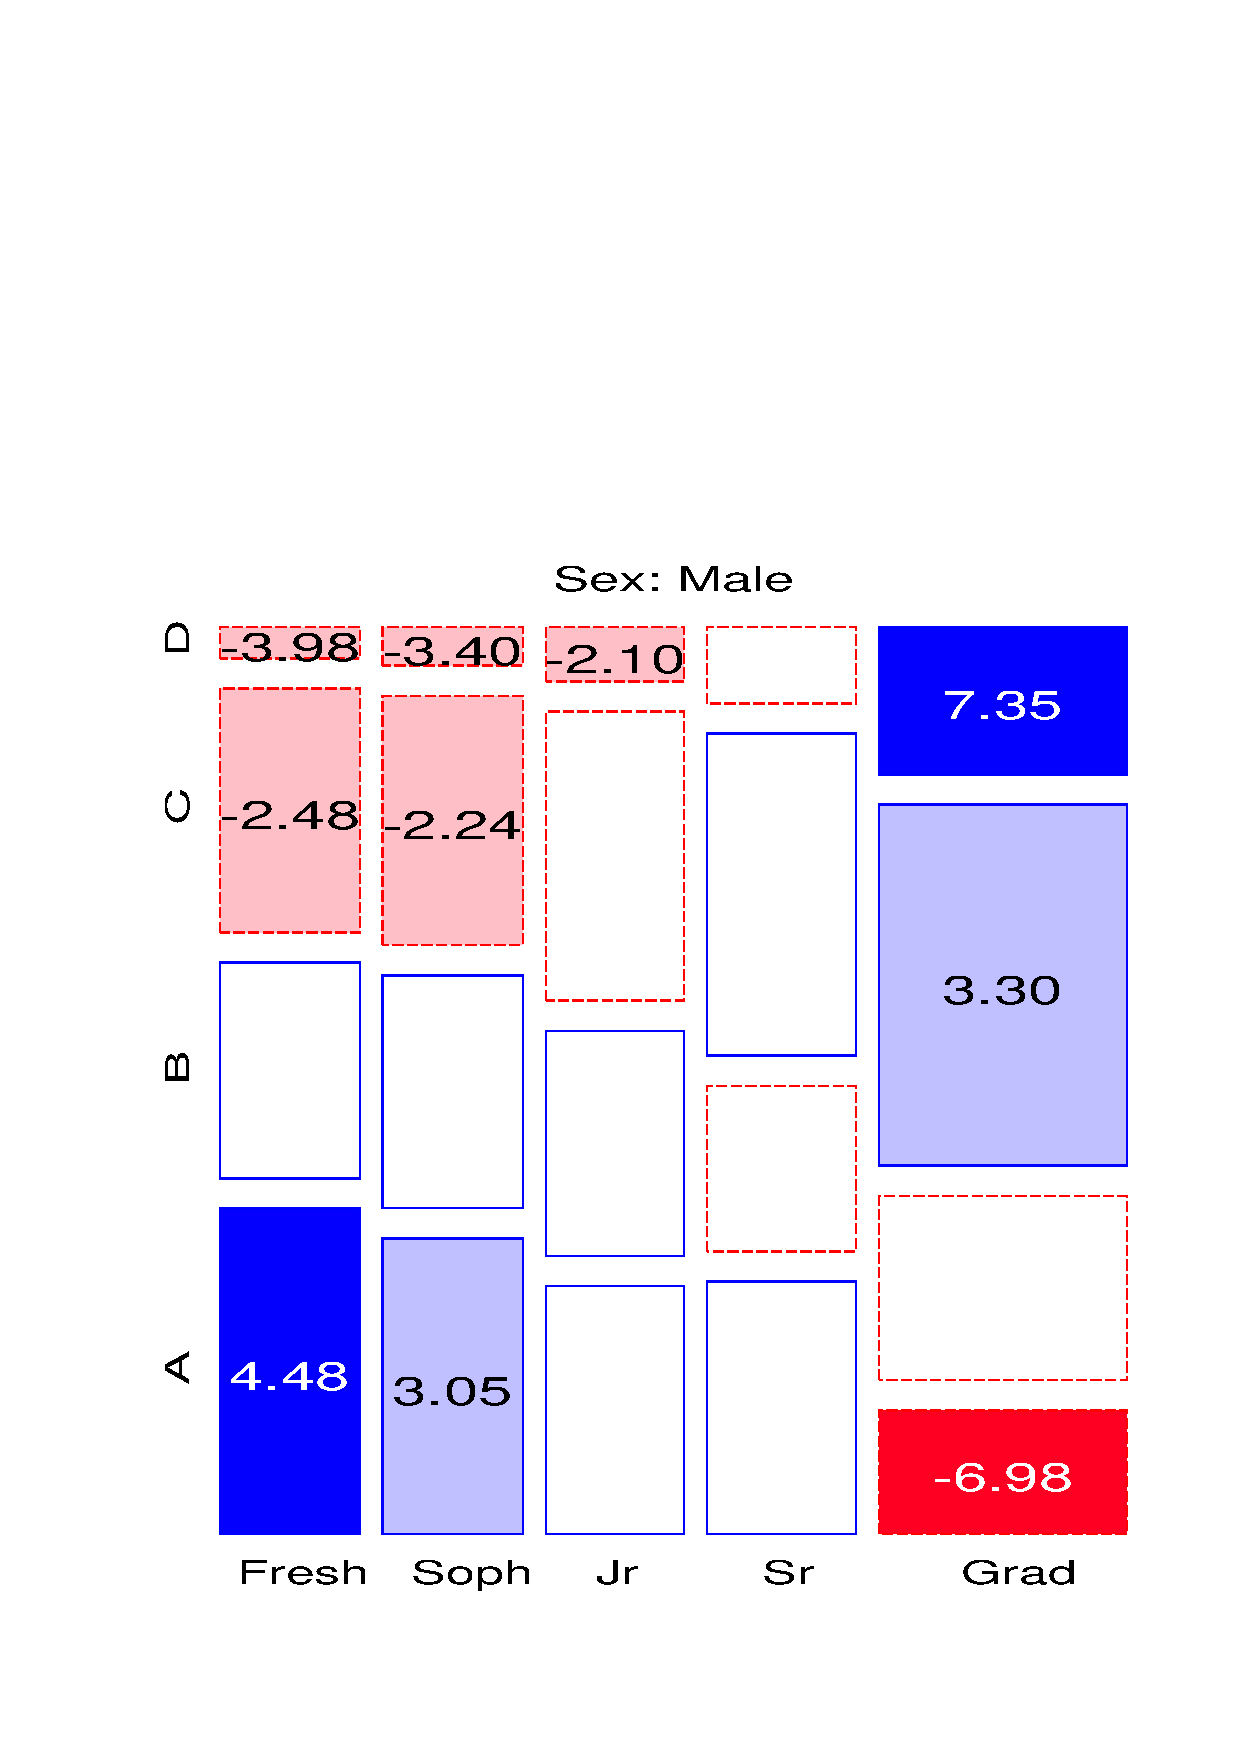
\includegraphics[width=1\linewidth,clip]{mosviet2}
 \end{minipage}
 \caption{Partial mosaic plots, by sex, for Vietnam war data}\label{fig:mosviet}
\end{figure}
With the variables in each mosaic ordered Year, Response,
recall that the height of each bar shows the (conditional) proportion
of students in each year who chose each response. There is no systematic
pattern for women, but the pattern of heights of the boxes, and of the
residuals from independence for men is very systematic.
The trend over years is easiest to see for responses A and D;
note that there is a large jump in proportion choosing these responses
between 4th year students and graduate students.
Perhaps our assumption of a linear trend with year for males needs
adjustment.

A \CA\ plot also displays residuals from a background model.  Here
we choose the null-response model of joint independence, $[SY] [R]$, so that all associations
between the response and the sex-year combinations will be shown.
To do this, we first transpose the data so that the responses
are columns and the sex-year populations are rows.
\begin{listing}
%include catdata(vietnam);

*-- Reshape to two-way table, SexYr x Response;
proc transpose data=vietnam prefix=R out=viet2way;
   var count;
   by sex year;

data viet2way;
   set viet2way;
   rename r1=A r2=B r3=C r4=D;
   sexyr = sex || put(year,1.);
   drop _name_;
proc print;

%corresp(data=viet2way, var=A--D, id=sexyr, interp=none join);
\end{listing}

The plot, shown in \figref{fig:vietcores} is quite revealing.
The response points, A--D
largely define the first dimension,
which accounts for 73.6\% of the association from the null-response model.
The year points for men, M1--M5,
are also ordered along this dimension, but male graduate students are far
from the male undergraduates.
The year points for women are tightly clustered, and aligned closest to
response C, their most preferred alternative.
The second dimension seems largely to do with the contrast between the relatively high choice for response D (``immediate withdrawal'')
among male graduate students and general preference for response C
(``de-escalate'') among most women.

%% one figure
\begin{figure}[htb]
  \centering
  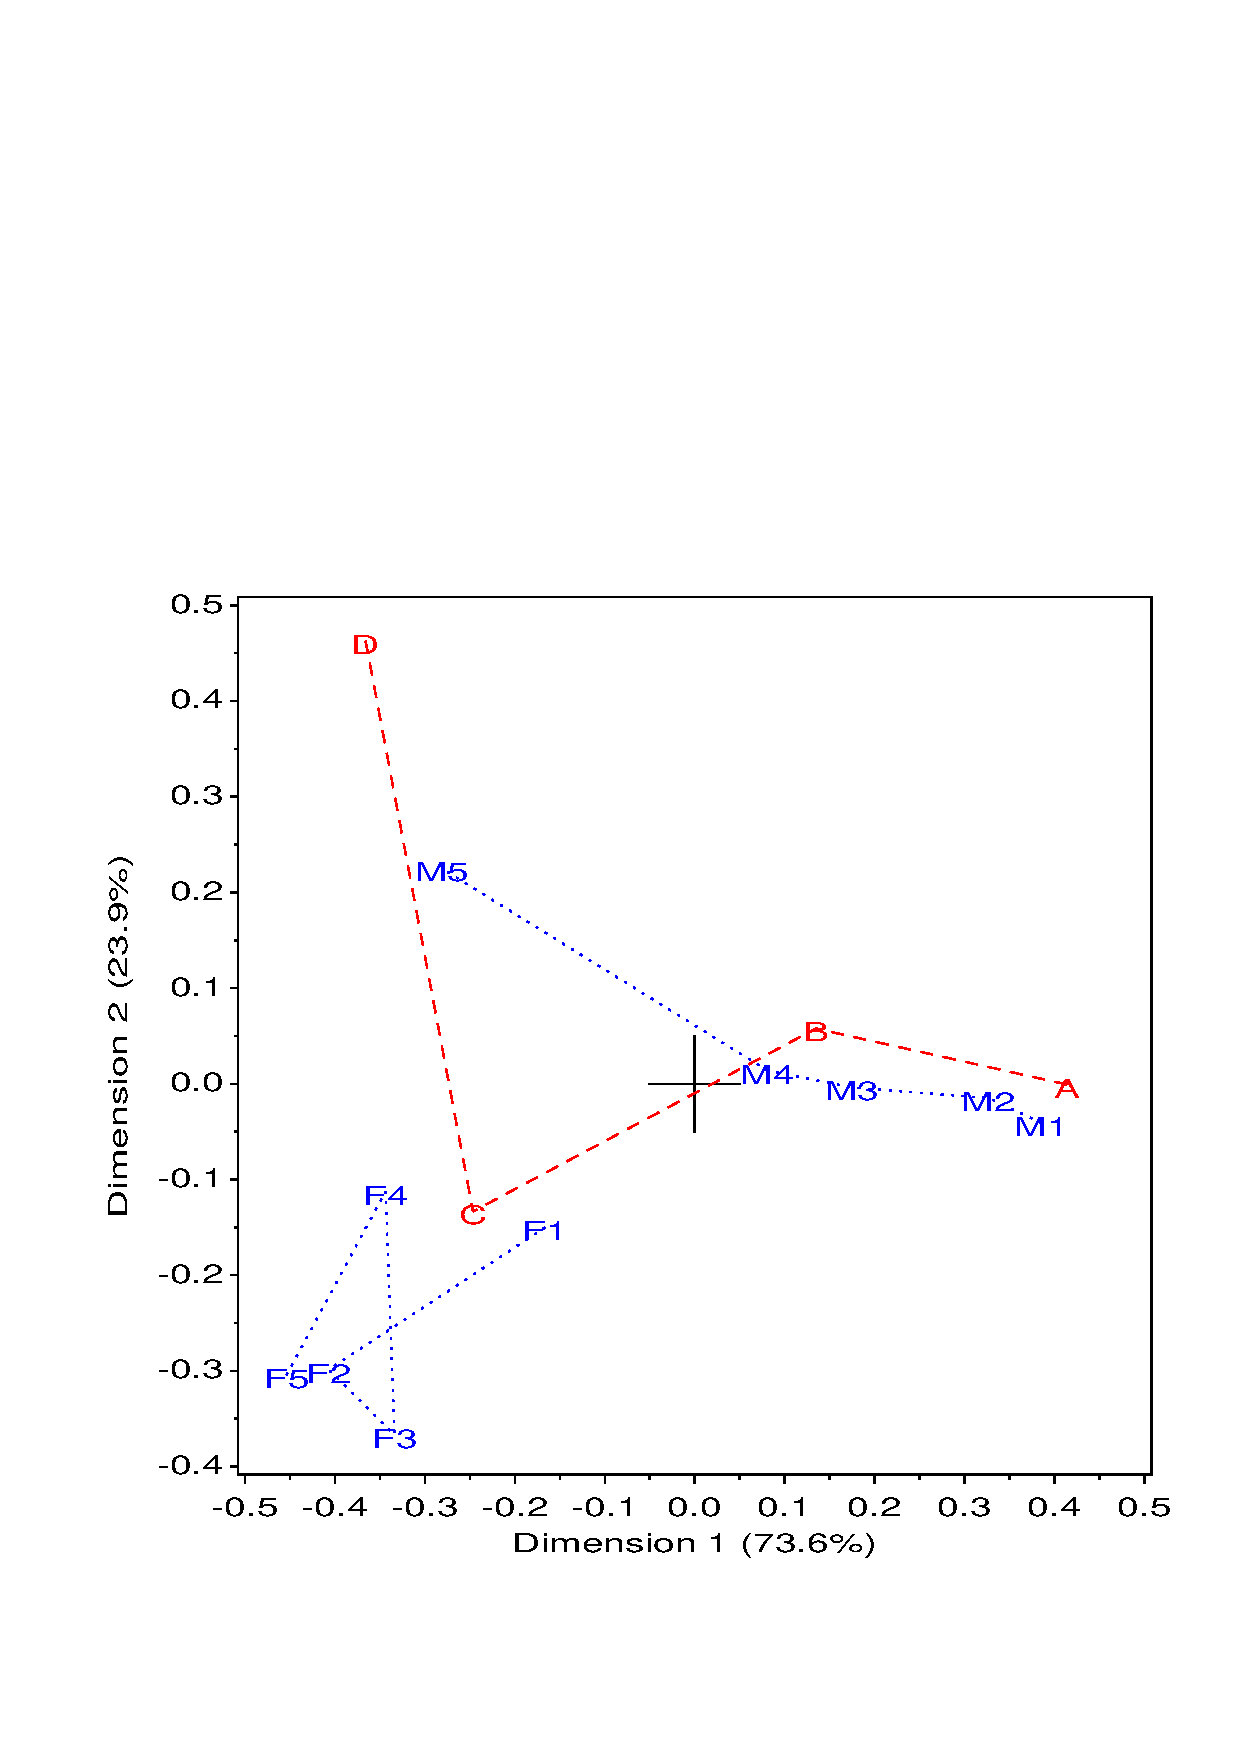
\includegraphics[scale=.6,clip]{vietcores}
  \caption{Correspondence analysis display for model $[SY][R]$}%
  \label{fig:vietcores}
\end{figure}

Both \figref{fig:mosviet} and \figref{fig:vietcores} indicate that our
assumption of linear spacing of year for men is incorrect, particularly
for graduate students.
A simple approach is to replace the variable \pname{year} with a new
variable, \pname{YR}, for which graduate students are some number
greater than 5.
Varying the year for graduate students over the range 5--10 gives
the residual \GSQ\ values (with 21 df)
in \tabref{tab:vietgrad}, and suggests that
7 years for graduate students gives the best fit.  The plot
of fitted and observed values under the revised model is shown in \figref{fig:vietnam3}.
\begin{Example}[vietnam3]{Student opinion about the Vietnam war}
The revised model, with linear effects of year on each logit,
and with graduate students treated as \pname{yr=7}
 shown in \figref{fig:vietnam3} was fit using
\PROC{CATMOD}.  However, influence diagnostics are
easier to obtain using
\PROC{GENMOD}.
The same model can be fit using \PROC{GENMOD} by defining a dummy variable
for women and an interaction between \pname{yr} and a dummy variable
for men.
\begin{listing}
data vietnam;
   set vietnam;
   yr = year + 2*(year=5);
   mlin =  yr * (sex='M');
   female = (sex='F');
   cell = trim(sex)|| put(year,1.)|| trim(put(response,letter.));
   label yr="Year + 2(Grad)";

proc genmod data=vietnam;
   class year sex response;
   model count = year|sex response|mlin  response|female /
         dist=poisson obstats residuals;
   make 'obstats' out=obstats;
\end{listing}
Normally, one would need to merge the input \Dset\ with the \pname{obstats},
and calculate hat values, Cook's D or other quantities for plotting:
\begin{listing}
%let k=8;
data obstats;
   merge vietnam obstats;
   h = hesswgt * std**2;
   cookd = streschi**2 * h/((1-h) * &k);
\end{listing}
where \pname{k=8} is the number of estimated parameters.

Instead, the \macro{INFLGLIM} (\macref{mac:inflglim}) automates these steps, and
gives various influence plots of residuals from a given
model.  The macro plots all combinations of the variables given
by the \mparm{GY}{INFLGLIM} against the variables given by the \mparm{GX}{INFLGLIM},
using a bubble symbol whose size is proportional to the
\mparm{BUBBLE}{INFLGLIM}, usually Cook's D.

Here, we plot the one-step estimates of change in deviance
($\Delta G_{(-i)}^2$, or \pname{DIFDEV})
due to deleting each cell against hat values,
using bubble symbols with area proportional to Cook's D.
The \mparm{infl}{INFLGLIM} determines the criterion for labeling
potentially influential points.
\begin{listing}
%inflglim(data=vietnam, resp=count,
    class=year sex response,
    model= year|sex  response|mlin  response|female,
    dist=poisson, id=cell,
    infl=%str(difdev>4 or &bubble>1 or hat>1.5*&hcrit),
    gy=difdev, gx=hat, bubble=cookd);
\end{listing}

This plot (\figref{fig:vietgen3}) shows that there are still two
large residuals: 4th year men choose response B substantially less often
than predicted (accounting for over one-third of the model deviance), and first year women choose response C less than
predicted.
%% one figure
\begin{figure}[htb]
  \centering
  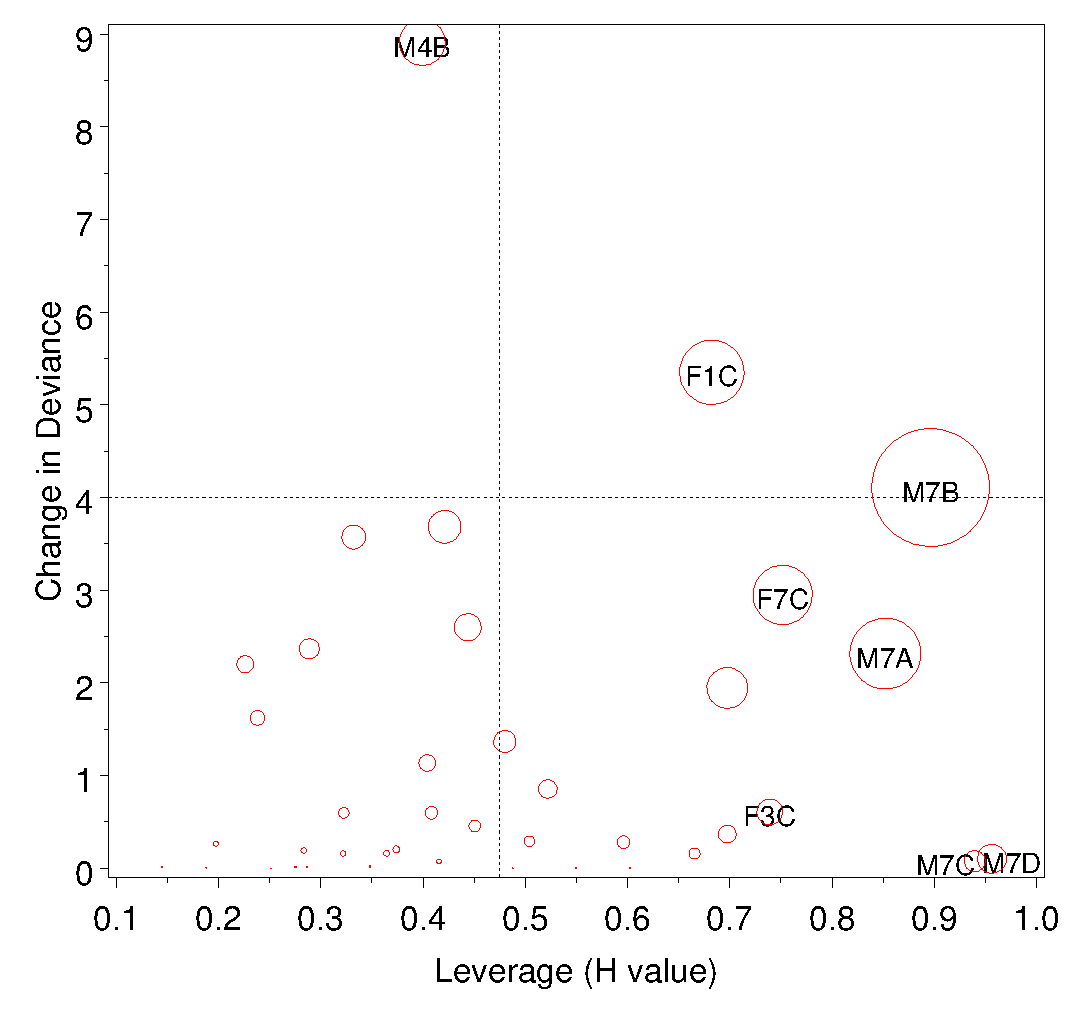
\includegraphics[scale=.6]{vietgen3}
  \caption{Influence plot for model $R = S + Y_{lin}(M)$, Graduate students=7}%
  \label{fig:vietgen3}
\end{figure}
We complete the analysis and this example with a half-normal plot of
these residuals, shown in \figref{fig:vietgen4}.  Although there is
evidence of non-normality in the distribution of residuals,  even the largest
values are within the simulated envelope.
\begin{listing}
%halfnorm(data=vietnam, resp=count,
   class=sex year response,
   model=year|sex  response|mlin  response|female,
   dist=poisson, id=cell);
\end{listing}

\begin{figure}[htb]
  \centering
  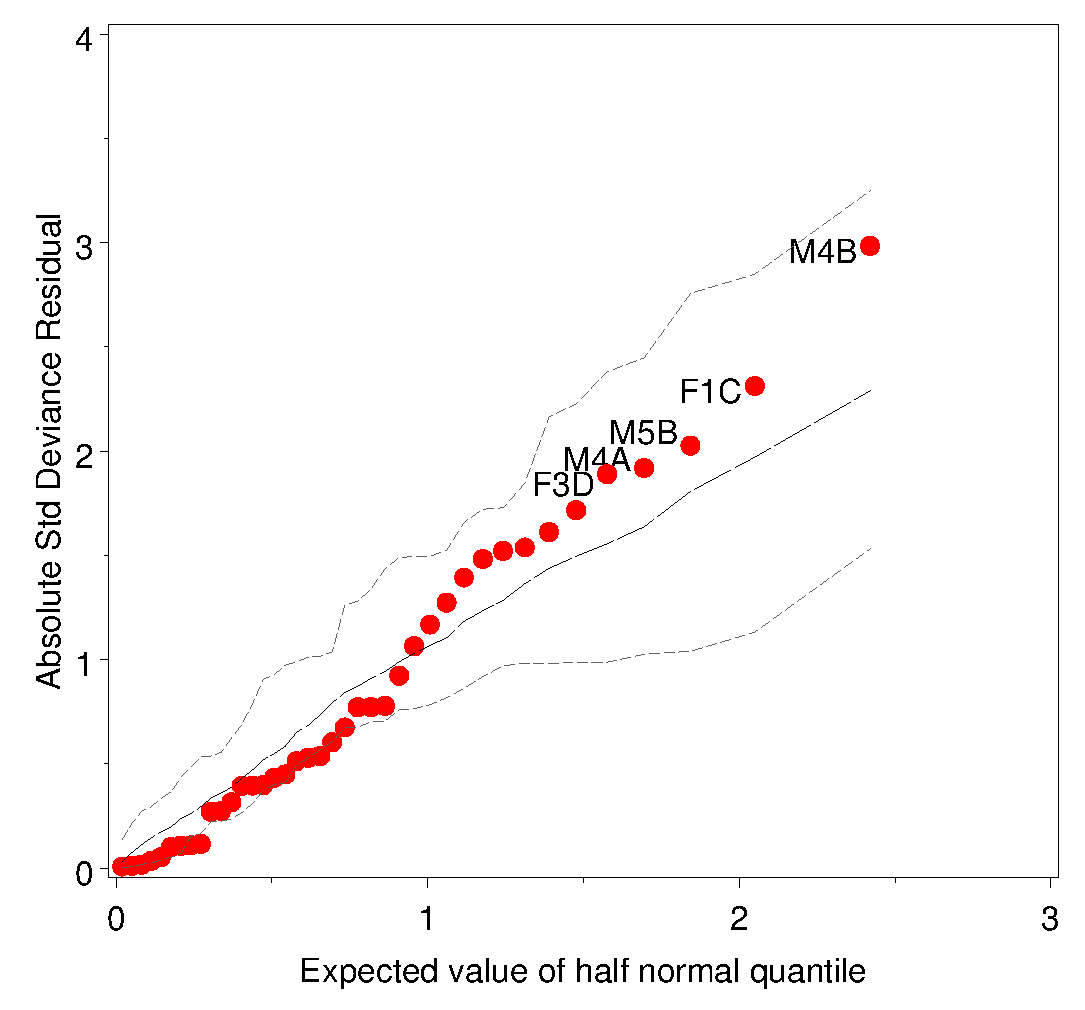
\includegraphics[scale=.6]{vietgen4}
  \caption{Half-normal plot for model $R = S + Y_{lin}(M)$, Graduate students=7}%
  \label{fig:vietgen4}
\end{figure}
\end{Example}

\begin{table}[htb]
 \caption{Profile deviance analysis of Year for Graduate Students}\label{tab:vietgrad}
 \begin{center}
 \begin{tabular}{cr}
  \hline
  Grad Year & \GSQ (21) \\
  \hline
  5 &  38.10 \\ 
  6 &  26.69 \\ 
  7 &  23.87 \\ 
  8 &  23.99 \\ 
  9 &  25.13 \\ 
  10 & 26.58 \\ 
  \hline
 \end{tabular}
 \end{center}
\end{table}


%% two subfig side-by-side
\begin{figure}[htb]
 \begin{minipage}[t]{.49\linewidth}
  \includegraphics[width=1\linewidth]{vietnam31}
 \end{minipage}%
 \hfill
 \begin{minipage}[t]{.49\linewidth}
  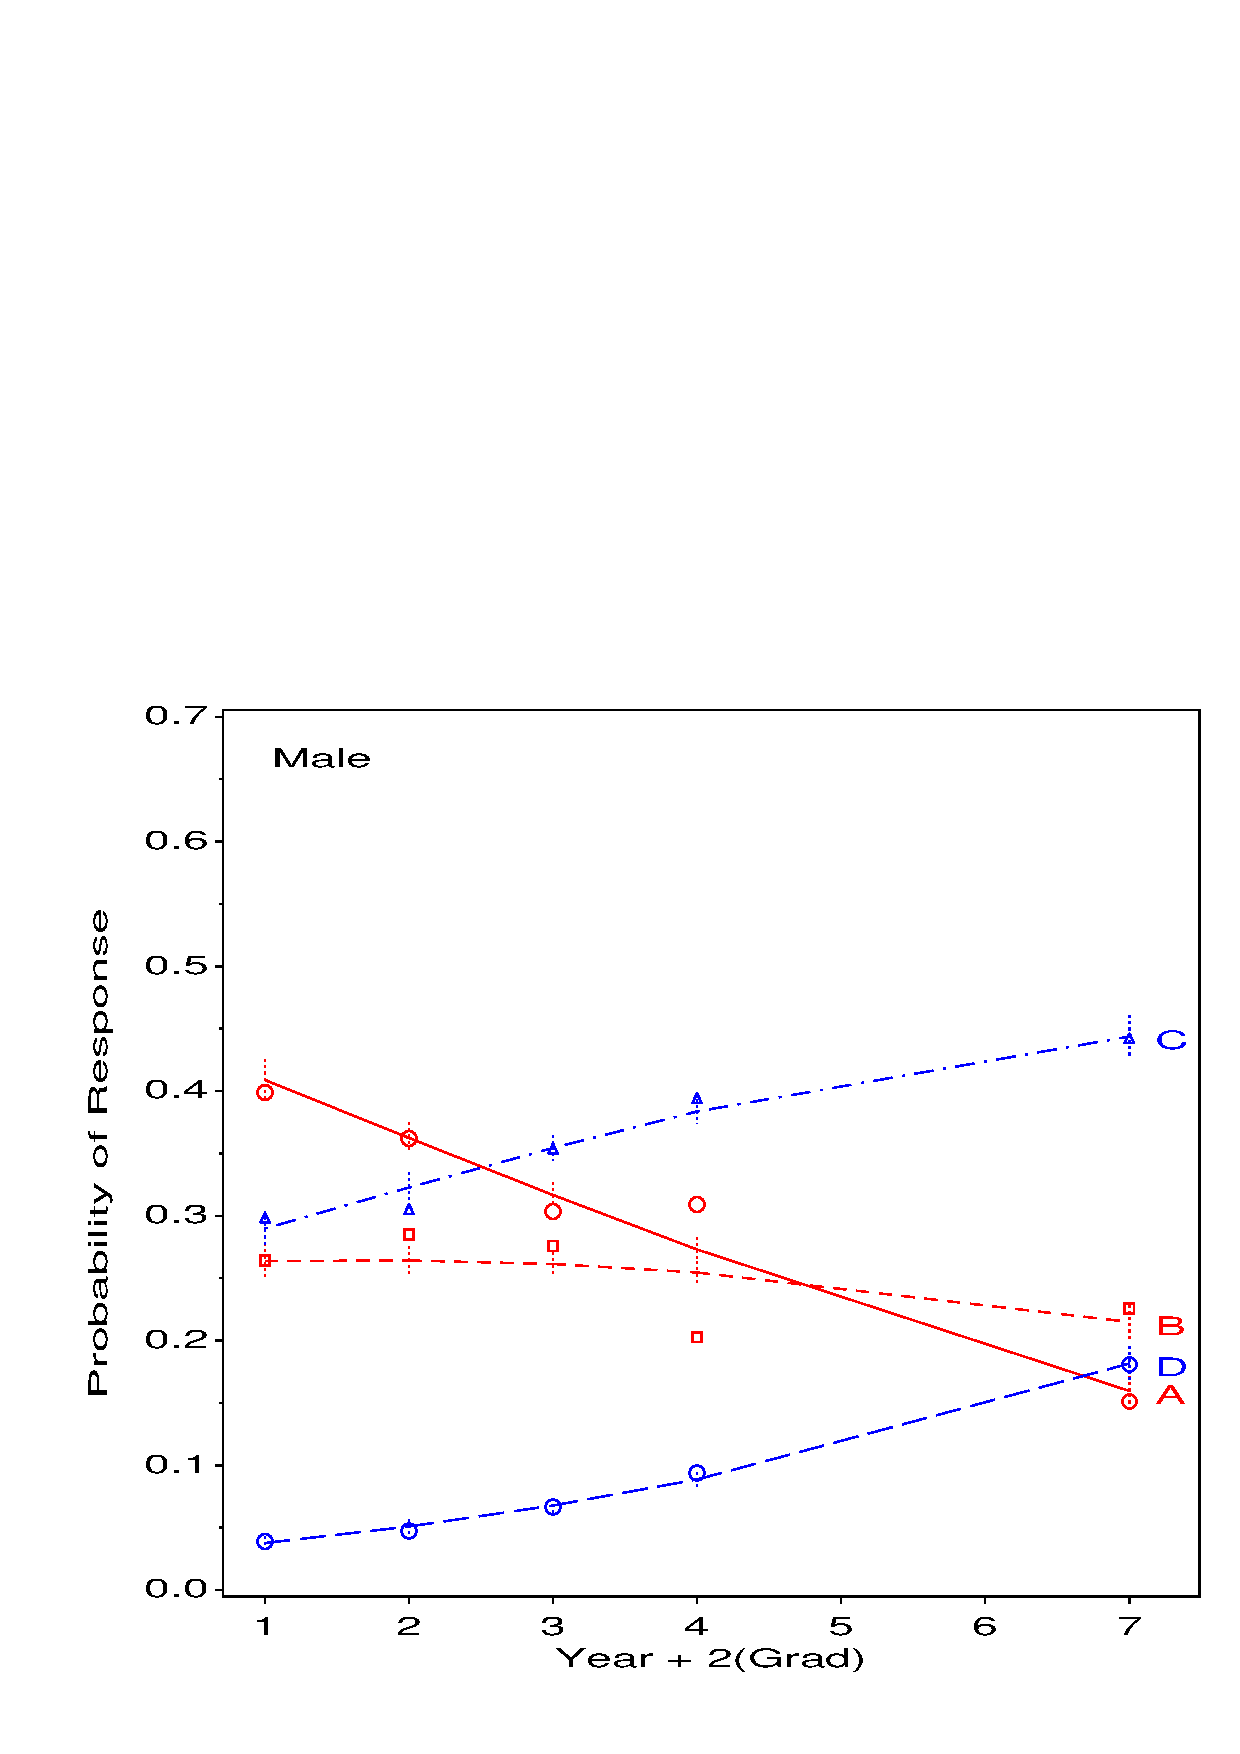
\includegraphics[width=1\linewidth]{vietnam32}
 \end{minipage}
 \caption{Observed and fitted probabilities for model $R = S + Y_{lin}(M)$, Graduate students=7}\label{fig:vietnam3}
\end{figure}

This model fits quite well overall, but there are still several
discrepant points.
We examine residuals and influence diagnostics for this model in
the following section
(\exref{ex:vietnam3}).
\end{Example}
